% Options for packages loaded elsewhere
\PassOptionsToPackage{unicode}{hyperref}
\PassOptionsToPackage{hyphens}{url}
%
\documentclass[
]{article}
\usepackage{ctex}
\usepackage{geometry}
\geometry{a4paper,left=2.8cm,right=2.8cm,top=3cm,bottom=2.5cm}
\usepackage{amsmath,amssymb}
\usepackage{graphicx}
\let\oldincludegraphics\includegraphics
\renewcommand{\includegraphics}[2][]{\begin{center}\oldincludegraphics[#1]{#2}\end{center}}
\usepackage{iftex}
\ifPDFTeX
  \usepackage[T1]{fontenc}
  \usepackage[utf8]{inputenc}
  \usepackage{textcomp} % provide euro and other symbols
\else % if luatex or xetex
  \usepackage{unicode-math} % this also loads fontspec
  \defaultfontfeatures{Scale=MatchLowercase}
  \defaultfontfeatures[\rmfamily]{Ligatures=TeX,Scale=1}
\fi
\usepackage{lmodern}
\ifPDFTeX\else
  % xetex/luatex font selection
\fi
% Use upquote if available, for straight quotes in verbatim environments
\IfFileExists{upquote.sty}{\usepackage{upquote}}{}
\IfFileExists{microtype.sty}{% use microtype if available
  \usepackage[]{microtype}
  \UseMicrotypeSet[protrusion]{basicmath} % disable protrusion for tt fonts
}{}
\makeatletter
\@ifundefined{KOMAClassName}{% if non-KOMA class
  \IfFileExists{parskip.sty}{%
    \usepackage{parskip}
  }{% else
    \setlength{\parindent}{0pt}
    \setlength{\parskip}{6pt plus 2pt minus 1pt}}
}{% if KOMA class
  \KOMAoptions{parskip=half}}
\makeatother
\usepackage{xcolor}
\usepackage{color}
\usepackage{fancyvrb}
\newcommand{\VerbBar}{|}
\newcommand{\VERB}{\Verb[commandchars=\\\{\}]}
\DefineVerbatimEnvironment{Highlighting}{Verbatim}{commandchars=\\\{\}}
% Add ',fontsize=\small' for more characters per line
\newenvironment{Shaded}{}{}
\newcommand{\AlertTok}[1]{\textcolor[rgb]{1.00,0.00,0.00}{\textbf{#1}}}
\newcommand{\AnnotationTok}[1]{\textcolor[rgb]{0.38,0.63,0.69}{\textbf{\textit{#1}}}}
\newcommand{\AttributeTok}[1]{\textcolor[rgb]{0.49,0.56,0.16}{#1}}
\newcommand{\BaseNTok}[1]{\textcolor[rgb]{0.25,0.63,0.44}{#1}}
\newcommand{\BuiltInTok}[1]{\textcolor[rgb]{0.00,0.50,0.00}{#1}}
\newcommand{\CharTok}[1]{\textcolor[rgb]{0.25,0.44,0.63}{#1}}
\newcommand{\CommentTok}[1]{\textcolor[rgb]{0.38,0.63,0.69}{\textit{#1}}}
\newcommand{\CommentVarTok}[1]{\textcolor[rgb]{0.38,0.63,0.69}{\textbf{\textit{#1}}}}
\newcommand{\ConstantTok}[1]{\textcolor[rgb]{0.53,0.00,0.00}{#1}}
\newcommand{\ControlFlowTok}[1]{\textcolor[rgb]{0.00,0.44,0.13}{\textbf{#1}}}
\newcommand{\DataTypeTok}[1]{\textcolor[rgb]{0.56,0.13,0.00}{#1}}
\newcommand{\DecValTok}[1]{\textcolor[rgb]{0.25,0.63,0.44}{#1}}
\newcommand{\DocumentationTok}[1]{\textcolor[rgb]{0.73,0.13,0.13}{\textit{#1}}}
\newcommand{\ErrorTok}[1]{\textcolor[rgb]{1.00,0.00,0.00}{\textbf{#1}}}
\newcommand{\ExtensionTok}[1]{#1}
\newcommand{\FloatTok}[1]{\textcolor[rgb]{0.25,0.63,0.44}{#1}}
\newcommand{\FunctionTok}[1]{\textcolor[rgb]{0.02,0.16,0.49}{#1}}
\newcommand{\ImportTok}[1]{\textcolor[rgb]{0.00,0.50,0.00}{\textbf{#1}}}
\newcommand{\InformationTok}[1]{\textcolor[rgb]{0.38,0.63,0.69}{\textbf{\textit{#1}}}}
\newcommand{\KeywordTok}[1]{\textcolor[rgb]{0.00,0.44,0.13}{\textbf{#1}}}
\newcommand{\NormalTok}[1]{#1}
\newcommand{\OperatorTok}[1]{\textcolor[rgb]{0.40,0.40,0.40}{#1}}
\newcommand{\OtherTok}[1]{\textcolor[rgb]{0.00,0.44,0.13}{#1}}
\newcommand{\PreprocessorTok}[1]{\textcolor[rgb]{0.74,0.48,0.00}{#1}}
\newcommand{\RegionMarkerTok}[1]{#1}
\newcommand{\SpecialCharTok}[1]{\textcolor[rgb]{0.25,0.44,0.63}{#1}}
\newcommand{\SpecialStringTok}[1]{\textcolor[rgb]{0.73,0.40,0.53}{#1}}
\newcommand{\StringTok}[1]{\textcolor[rgb]{0.25,0.44,0.63}{#1}}
\newcommand{\VariableTok}[1]{\textcolor[rgb]{0.10,0.09,0.49}{#1}}
\newcommand{\VerbatimStringTok}[1]{\textcolor[rgb]{0.25,0.44,0.63}{#1}}
\newcommand{\WarningTok}[1]{\textcolor[rgb]{0.38,0.63,0.69}{\textbf{\textit{#1}}}}
\usepackage{longtable,booktabs,array}
\usepackage{calc} % for calculating minipage widths
% Correct order of tables after \paragraph or \subparagraph
\usepackage{etoolbox}
\makeatletter
\patchcmd\longtable{\par}{\if@noskipsec\mbox{}\fi\par}{}{}
\makeatother
% Allow footnotes in longtable head/foot
\IfFileExists{footnotehyper.sty}{\usepackage{footnotehyper}}{\usepackage{footnote}}
\makesavenoteenv{longtable}
\usepackage{graphicx}
\makeatletter
\def\maxwidth{\ifdim\Gin@nat@width>\linewidth\linewidth\else\Gin@nat@width\fi}
\def\maxheight{\ifdim\Gin@nat@height>\textheight\textheight\else\Gin@nat@height\fi}
\makeatother
% Scale images if necessary, so that they will not overflow the page
% margins by default, and it is still possible to overwrite the defaults
% using explicit options in \includegraphics[width, height, ...]{}
\setkeys{Gin}{width=0.5\textwidth,keepaspectratio}
% Set default figure placement to htbp
\makeatletter
\def\fps@figure{htbp}
\makeatother
\setlength{\emergencystretch}{3em} % prevent overfull lines
\providecommand{\tightlist}{%
  \setlength{\itemsep}{0pt}\setlength{\parskip}{0pt}}
\setcounter{secnumdepth}{-\maxdimen} % remove section numbering
\ifLuaTeX
  \usepackage{selnolig}  % disable illegal ligatures
\fi
\IfFileExists{bookmark.sty}{\usepackage{bookmark}}{\usepackage{hyperref}}
\IfFileExists{xurl.sty}{\usepackage{xurl}}{} % add URL line breaks if available
\urlstyle{same}
\hypersetup{
  hidelinks,
  pdfcreator={LaTeX via pandoc}}

\author{}
\date{}

\begin{document}
\pagenumbering{Roman}
\hypertarget{review-of-the-course-r-for-data-science-part-03talk-09-12}{%
\section{Review of the course ``R for Data Science'' Part 03(Talk
09\textasciitilde{}
12)}\label{review-of-the-course-r-for-data-science-part-03talk-09-12}}

\textbf{By Haoran Nie @ HUST Life ST}

\textbf{Partically translated by
\href{https://github.com/1508324011}{Rui Zhu @ HUST Life ST}}

\textbf{双语版}

This work is licensed under CC BY-NC-SA 4.0

\begin{center}\rule{0.5\linewidth}{0.5pt}\end{center}
\tableofcontents

\newpage
\pagenumbering{arabic}
\hypertarget{r-for-bioinformatics-data-visualisation}{%
\section{R for bioinformatics, data
visualisation}\label{r-for-bioinformatics-data-visualisation}}

\begin{quote}
Talk 09
\end{quote}

\hypertarget{toc}{%
\subsection{TOC}\label{toc}}

\begin{itemize}
\item
  basic plot functions
\item
  basic \texttt{ggplot2}
\item
  special letters
\item
  equations
\item
  advanced \texttt{ggplot2}
\end{itemize}

\hypertarget{basic-plot-functions-using-r}{%
\subsection{Basic plot functions using
R}\label{basic-plot-functions-using-r}}

\hypertarget{dot-plot-ux6563ux70b9ux56fe}{%
\subsubsection{Dot plot 散点图}\label{dot-plot-ux6563ux70b9ux56fe}}

\textbf{An example:}

\begin{Shaded}
\begin{Highlighting}[]
\FunctionTok{with}\NormalTok{( }
\NormalTok{  swiss,}
  \CommentTok{\#将数据框 swiss 中的列作为环境,可以直接使用列名而不需要再加上swiss\$前缀。 }
  \FunctionTok{plot}\NormalTok{(}
\NormalTok{    Education, }
\NormalTok{    Fertility,}
    \AttributeTok{type =} \StringTok{"p"}\NormalTok{, }
    \AttributeTok{main =} \StringTok{"Swiss data 1888"}\NormalTok{, }
    \AttributeTok{sub =} \StringTok{"Socioeconomic indicators \& Fertility"}\NormalTok{, }
    \AttributeTok{xlab =} \StringTok{"Education"}\NormalTok{, }
    \AttributeTok{ylab =} \StringTok{"Fertility"}\NormalTok{, }
    \AttributeTok{col =} \StringTok{"darkblue"}\NormalTok{, }
    \AttributeTok{xlim =} \FunctionTok{range}\NormalTok{( Education ), }
    \AttributeTok{ylim =} \FunctionTok{range}\NormalTok{( Fertility ), }
    \AttributeTok{pch =} \DecValTok{20}\NormalTok{, }
    \AttributeTok{frame.plot =}\NormalTok{ F}\DocumentationTok{\#\#去除图的边框}
\NormalTok{  ) }
\NormalTok{)}
\end{Highlighting}
\end{Shaded}

\includegraphics{/Users/lucas/Library/Mobile Documents/com~apple~CloudDocs/~~aa Study Materials/Grade 2 I/Learning/R for Data Science/Review of R/markdown/image/image-20231212160107785.png}

\textbf{Function usage:}

\begin{Shaded}
\begin{Highlighting}[]
\DocumentationTok{\#\# Default S3 method:}
\FunctionTok{plot}\NormalTok{(}
\NormalTok{  x, }
\NormalTok{  y, }
  \AttributeTok{type =} \StringTok{"p"}\NormalTok{, }
  \AttributeTok{xlim =} \ConstantTok{NULL}\NormalTok{, }\AttributeTok{ylim =} \ConstantTok{NULL}\NormalTok{,}
  \AttributeTok{log =} \StringTok{""}\NormalTok{, }
  \AttributeTok{main =} \ConstantTok{NULL}\NormalTok{, }\AttributeTok{sub =} \ConstantTok{NULL}\NormalTok{, }
  \AttributeTok{xlab =} \ConstantTok{NULL}\NormalTok{, }\AttributeTok{ylab =} \ConstantTok{NULL}\NormalTok{,}
  \AttributeTok{ann =} \FunctionTok{par}\NormalTok{(}\StringTok{"ann"}\NormalTok{), }\DocumentationTok{\#\#par("ann")=T}
  \AttributeTok{axes =} \ConstantTok{TRUE}\NormalTok{, }\AttributeTok{frame.plot =}\NormalTok{ axes,}
  \AttributeTok{panel.first =} \ConstantTok{NULL}\NormalTok{, }\AttributeTok{panel.last =} \ConstantTok{NULL}\NormalTok{, }\AttributeTok{asp =} \ConstantTok{NA}\NormalTok{,}
  \AttributeTok{xgap.axis =} \ConstantTok{NA}\NormalTok{, }\AttributeTok{ygap.axis =} \ConstantTok{NA}\NormalTok{,}
\NormalTok{  ...}
\NormalTok{)}
\CommentTok{\# Default Parameters are listed.}
\end{Highlighting}
\end{Shaded}

\textbf{Arguments}

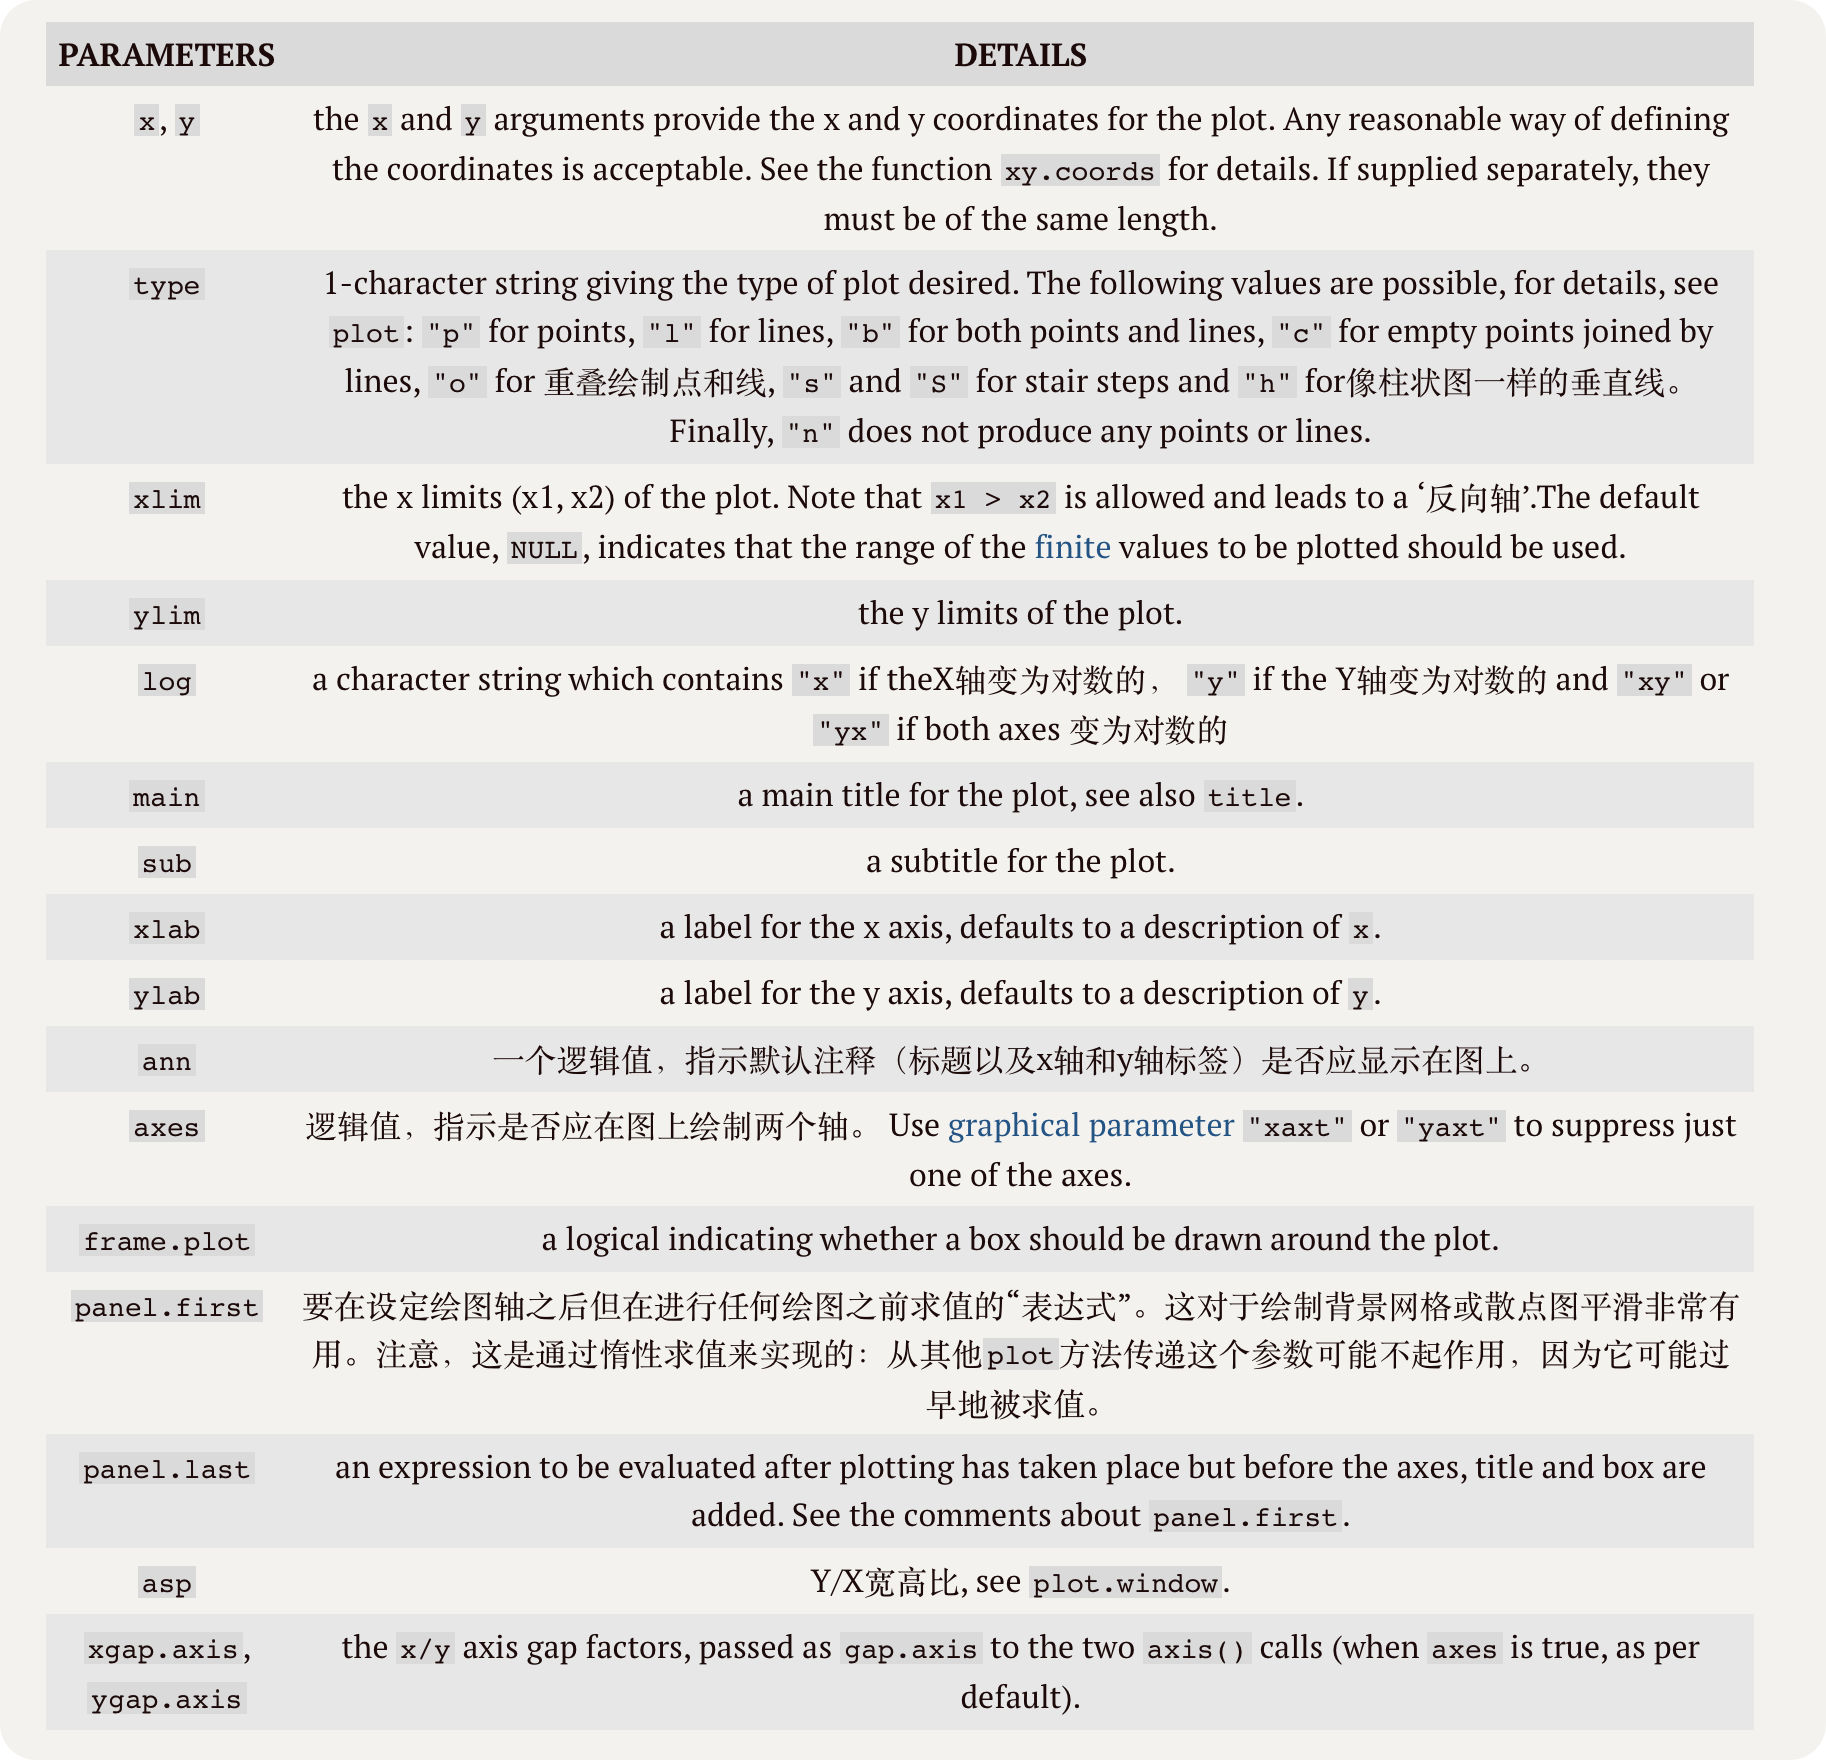
\includegraphics[width=0.8\textwidth]{/Users/lucas/Library/Mobile Documents/com~apple~CloudDocs/~~aa Study Materials/Grade 2 I/Learning/R for Data Science/Review of R/markdown/image/image-20231213063700615.png}

You can also use \texttt{ggplot} to draw the plot above:

\begin{Shaded}
\begin{Highlighting}[]
\FunctionTok{ggplot}\NormalTok{( }
\NormalTok{  swiss, }
  \FunctionTok{aes}\NormalTok{(}\AttributeTok{x =}\NormalTok{ Education, }\AttributeTok{y =}\NormalTok{ Fertility) }
\NormalTok{) }\SpecialCharTok{+} 
\FunctionTok{geom\_point}\NormalTok{() }\SpecialCharTok{+} 
\FunctionTok{scale\_x\_log10}\NormalTok{() }\SpecialCharTok{+} 
\FunctionTok{scale\_y\_log10}\NormalTok{() }\SpecialCharTok{+} 
\FunctionTok{xlab}\NormalTok{(}\StringTok{"Education"}\NormalTok{) }\SpecialCharTok{+} 
\FunctionTok{ylab}\NormalTok{(}\StringTok{"Fertility"}\NormalTok{) }\SpecialCharTok{+} 
\NormalTok{ggtitle }\StringTok{"Swiss data 1888"}\ErrorTok{)}
\end{Highlighting}
\end{Shaded}

\hypertarget{high-level-and-low-level}{%
\subsubsection{High-level and
low-level}\label{high-level-and-low-level}}

\begin{itemize}
\item
  \textbf{high level}: 绘图函数在图形设备上创建新的绘图
\item
  \textbf{low level}:绘图函数向现有绘图添加更多信息
\end{itemize}

\hypertarget{low-level-plots}{%
\paragraph{Low level plots}\label{low-level-plots}}

\begin{itemize}
\item
  \texttt{points} : 点图
\item
  \texttt{lines} : 线图
\item
  \texttt{abline} : 直线
\item
  \texttt{polygon} : 多边形
\item
  \texttt{legend} : 图例
\item
  \texttt{title} : 标题
\item
  \texttt{axis} : 轴
\end{itemize}

\hypertarget{high-level-plots}{%
\paragraph{High level plots}\label{high-level-plots}}

\begin{itemize}
\item
  \texttt{plot} : 通用画图函数
\item
  \texttt{pairs}
\item
  \texttt{coplot}
\item
  \texttt{qqnorm}
\item
  \texttt{hist}
\item
  \texttt{dotchart}
\item
  \texttt{image}
\item
  \texttt{contour}
\end{itemize}

\textbf{注}: 可以用 \texttt{add\ =\ TRUE} 参数(如果可用)将 high level
函数强制转换为 low level

\hypertarget{ux56feux5f62ux76f8ux5173ux53c2ux6570ux7cfbux7edfux51fdux6570uxff09}{%
\subsubsection{图形相关参数(系统函数)}\label{ux56feux5f62ux76f8ux5173ux53c2ux6570ux7cfbux7edfux51fdux6570uxff09}}

\texttt{par()} 函数:
显示或修改当前\textbf{图形设备}的参数。用以下命令查看支持的内容:

\begin{Shaded}
\begin{Highlighting}[]
\FunctionTok{par}\NormalTok{( }\FunctionTok{c}\NormalTok{( }\StringTok{"mar"}\NormalTok{, }\StringTok{"bg"}\NormalTok{ ) ); }\DocumentationTok{\#\# 显示指定参数的值}
\DocumentationTok{\#\# 显示所有参数 }
\FunctionTok{par}\NormalTok{(); }
\end{Highlighting}
\end{Shaded}

\hypertarget{ux8c03ux6574-par-ux53c2ux6570ux524dux8bf7ux5907ux4efd}{%
\subsubsection{\texorpdfstring{调整 \texttt{par()}
参数前请备份}{调整 par() 参数前请备份}}\label{ux8c03ux6574-par-ux53c2ux6570ux524dux8bf7ux5907ux4efd}}

\texttt{par()} 用于指定全局参数,因此在改变前尽量备份

\begin{Shaded}
\begin{Highlighting}[]
\NormalTok{oldpar }\OtherTok{\textless{}{-}} \FunctionTok{par}\NormalTok{(); }\DocumentationTok{\#\# 备份}

\NormalTok{do some changes here ... }

\DocumentationTok{\#\# 恢复}
\FunctionTok{par}\NormalTok{( oldpar ); }
\end{Highlighting}
\end{Shaded}

\hypertarget{ux5e38ux7528ux56feux5f62ux53c2ux6570ux53caux8c03ux6574-margin}{%
\subsubsection{常用图形参数及调整:
margin}\label{ux5e38ux7528ux56feux5f62ux53c2ux6570ux53caux8c03ux6574-margin}}

图形边距( figure margins )

分别指定 下 -\textgreater{} 左 -\textgreater{} 上 -\textgreater{} 右
的边距,即从下面开始,顺时针移动。

\begin{Shaded}
\begin{Highlighting}[]
\CommentTok{\#单位是: text lines  }
\FunctionTok{par}\NormalTok{( }\AttributeTok{mar =} \FunctionTok{c}\NormalTok{( }\FloatTok{5.1}\NormalTok{, }\FloatTok{4.1}\NormalTok{, }\FloatTok{4.1}\NormalTok{, }\FloatTok{2.1}\NormalTok{ )); }\DocumentationTok{\#\# 设置新 martin}
\CommentTok{\#单位是: inch }
\FunctionTok{par}\NormalTok{( }\AttributeTok{mai =} \FunctionTok{c}\NormalTok{( }\FloatTok{5.1}\NormalTok{, }\FloatTok{4.1}\NormalTok{, }\FloatTok{4.1}\NormalTok{, }\FloatTok{2.1}\NormalTok{ )); }\DocumentationTok{\#\# 设置新 martin}
\end{Highlighting}
\end{Shaded}

\hypertarget{ux5e38ux7528ux56feux5f62ux53c2ux6570ux53caux8c03ux6574-ux591apanel}{%
\subsubsection{\texorpdfstring{常用图形参数及调整: 多panel
}{常用图形参数及调整: 多panel }}\label{ux5e38ux7528ux56feux5f62ux53c2ux6570ux53caux8c03ux6574-ux591apanel}}

画 2x3 共 6个panel,从左到右。(2行3列)

\begin{Shaded}
\begin{Highlighting}[]
\FunctionTok{par}\NormalTok{( }\AttributeTok{mfrow=}\FunctionTok{c}\NormalTok{(}\DecValTok{2}\NormalTok{,}\DecValTok{3}\NormalTok{) );}
\ControlFlowTok{for}\NormalTok{( i }\ControlFlowTok{in} \DecValTok{1}\SpecialCharTok{:}\DecValTok{6}\NormalTok{ )}
  \FunctionTok{plot}\NormalTok{( }\FunctionTok{sample}\NormalTok{( }\DecValTok{1}\SpecialCharTok{:}\DecValTok{10}\NormalTok{, }\DecValTok{10}\NormalTok{ ), }\AttributeTok{main =}\NormalTok{ i );}
\end{Highlighting}
\end{Shaded}

画 2x3 共 6个panel,从上到下。(2行3列)

\begin{Shaded}
\begin{Highlighting}[]
\FunctionTok{par}\NormalTok{( }\AttributeTok{mfcol=}\FunctionTok{c}\NormalTok{(}\DecValTok{2}\NormalTok{,}\DecValTok{3}\NormalTok{) );}
\ControlFlowTok{for}\NormalTok{( i }\ControlFlowTok{in} \DecValTok{1}\SpecialCharTok{:}\DecValTok{6}\NormalTok{ )}
  \FunctionTok{plot}\NormalTok{( }\FunctionTok{sample}\NormalTok{( }\DecValTok{1}\SpecialCharTok{:}\DecValTok{10}\NormalTok{, }\DecValTok{10}\NormalTok{ ), }\AttributeTok{main =}\NormalTok{ i );}
\end{Highlighting}
\end{Shaded}

\hypertarget{ux91cdux8981ux6982ux5ff5ux56feux5f62ux8bbeux5907}{%
\subsubsection{重要概念:图形设备}\label{ux91cdux8981ux6982ux5ff5ux56feux5f62ux8bbeux5907}}

\textbf{图形设备}是指图形输出的设备,可以将\textbf{图形设备}理解为\textbf{保存格式}
。

默认设备是:

\begin{itemize}
\item
  X11() : Unix
\item
  windows() : windows
\item
  quartz() : OS X
\end{itemize}

图形显示在\textbf{显示器}上。

\hypertarget{ux56feux5f62ux8bbeux5907cont}{%
\subsubsection{\texorpdfstring{图形设备:cont.
}{图形设备:cont. }}\label{ux56feux5f62ux8bbeux5907cont}}

常用其它设备有:

\begin{itemize}
\item
  pdf()
\item
  png()
\item
  jpeg()
\end{itemize}

分别对应输出文件格式。

\hypertarget{ux5e38ux7528ux56feux5f62ux8bbeux5907-pdf}{%
\subsubsection{\texorpdfstring{常用图形设备: pdf()
}{常用图形设备: pdf() }}\label{ux5e38ux7528ux56feux5f62ux8bbeux5907-pdf}}

使用方法如下:

\begin{Shaded}
\begin{Highlighting}[]
\FunctionTok{pdf}\NormalTok{( }\AttributeTok{file =} \StringTok{"/path/to/dir/\textless{}file\_name\textgreater{}.pdf"}\NormalTok{, }\AttributeTok{height =} \DecValTok{5}\NormalTok{, }\AttributeTok{width =} \DecValTok{5}\NormalTok{ ); }\DocumentationTok{\#\# 创建一个新设备/ pdf 文件 }
\FunctionTok{plot}\NormalTok{(}\DecValTok{1}\SpecialCharTok{:}\DecValTok{10}\NormalTok{); }\DocumentationTok{\#\# 作图;}
\FunctionTok{dev.off}\NormalTok{(); }\DocumentationTok{\#\# 关闭设备}
\end{Highlighting}
\end{Shaded}

\textbf{说明}

\begin{enumerate}
\def\labelenumi{\arabic{enumi}.}
\item
  默认文件名为 \texttt{Rplots.pdf} ,
\item
  \texttt{dev.off()} 必须关闭。关闭后,返回到最近使用的图形设备
\item
  \texttt{height} 和 \texttt{width} 参数的单位是 inch
\item
  如果运行多个 high level 作图命令,则会产生\textbf{多页pdf}
\end{enumerate}

\hypertarget{ux8bf7ux5c3dux91cfux4f7fux7528-pdf-ux4f5cux4e3aux6587ux4ef6ux8f93ux51faux683cux5f0f}{%
\subsubsection{请尽量使用 pdf
作为文件输出格式}\label{ux8bf7ux5c3dux91cfux4f7fux7528-pdf-ux4f5cux4e3aux6587ux4ef6ux8f93ux51faux683cux5f0f}}

\begin{enumerate}
\def\labelenumi{\arabic{enumi}.}
\item
  生信图片大多是点线图,适合保存为矢量格式(如pdf, ps 等);
\item
  矢量图可无限放大而不失真(变成像素);
\item
  可由 Adobe Illustrator 等矢量图软件进行编辑
\end{enumerate}

\hypertarget{ggplot2}{%
\subsection{\texorpdfstring{\texttt{ggplot2}}{ggplot2}}\label{ggplot2}}

You should know that

\begin{enumerate}
\def\labelenumi{\arabic{enumi}.}
\item
  \texttt{xy\ -axes} will automatically adjust based on the data you
  give;
\item
  \texttt{ggplot2} plotting results can be saved in variables and more
  layers can be added;
\item
  Layers using their own data need to be specified with
  \texttt{data\ =}, while global data is not. You can just specify it
  via \texttt{ggplot(data\ =\ data.frame(...))}.
\end{enumerate}

\hypertarget{some-basic-parameters-of-ggplot2}{%
\subsubsection{\texorpdfstring{Some basic parameters of
\texttt{ggplot2}}{Some basic parameters of ggplot2}}\label{some-basic-parameters-of-ggplot2}}

\begin{enumerate}
\def\labelenumi{\arabic{enumi}.}
\item
  \textbf{aes}
  (aesthetics)美学:控制全局参数,包括:x,y轴使用的数据,颜色( colour,
  fill) ,形状 ( shape ),大小 ( size ),分组 ( group ) 等等;
\item
  \textbf{图层}: \texttt{geom\_\textless{}layer\_name\textgreater{}}
  ;每张图可有多个图层(此处有两个);图层可使用全局数据 (df) 和参数
  (aes),也可以使用自己的 aes 和 数据;

  \texttt{geom\_\textless{}name\_of\_the\_layer\textgreater{}}:
\end{enumerate}

\begin{itemize}
\item
  \texttt{geom\_point} , \texttt{geom\_line}:
  点线图,用于揭示两组数据间的关系;
\end{itemize}

\begin{itemize}
\item
  \texttt{geom\_smooth} : 常与 \texttt{geom\_point}
  联合使用,揭示数据走势
\item
  \texttt{geom\_bar} : bar 图
\item
  \texttt{geom\_boxplot} : 箱线图,用于比较N组数据,揭示区别
\item
  \texttt{geom\_path} : 与\texttt{geom\_line}
  相似,但也可以画其它复杂图形
\item
  \texttt{geom\_histogram}, `` geom\_density ``` :
  数据的分布,也可用于多组间的比较
\item
  \ldots\ldots{}
\end{itemize}

\begin{enumerate}
\def\labelenumi{\arabic{enumi}.}
\item
  \texttt{scale} - Display Control其它控制函数

  \texttt{scale\_\textless{}控制内容\textgreater{}\_\textless{}控制手段\textgreater{}},

  e.g. \texttt{scale\_color\_manual()}: 以\textbf{手选方式} 控制
  \textbf{颜色}
\end{enumerate}

\begin{itemize}
\item
  \texttt{scale\_color\_...}

  \begin{itemize}
  \item
    \texttt{...\_gradient()}: 为不同数量的变量及其颜色使用渐变色。

    \begin{itemize}
    \item
      \texttt{...\_gradient2()}
    \item
      \texttt{...\_gradientn()}
    \end{itemize}
  \item
    \texttt{...\_brewer}: 使用默认调色板。
  \end{itemize}
\item
  \texttt{scale\_fill\_...}

  \begin{itemize}
  \item
    \textbf{\texttt{scale\_fill\_manual()}}:允许用户手动指定每个类别或组的填充颜色。
  \item
    \textbf{\texttt{scale\_fill\_discrete()}}:用于离散变量,自动为每个类别分配不同的颜色。
  \item
    \textbf{\texttt{scale\_fill\_continuous()}}:用于连续变量,根据连续数值分配颜色。
  \item
    \textbf{\texttt{scale\_fill\_gradient()}}、

    \textbf{\texttt{scale\_fill\_gradient2()}}、

    \textbf{\texttt{scale\_fill\_gradientn()}}:用于创建渐变颜色填充,适用于表示连续数值范围。
  \end{itemize}
\item
  \texttt{scale\_shape\_...}

  \begin{itemize}
  \item
    \textbf{\texttt{scale\_shape\_manual()}}:允许用户手动指定每个因子水平的形状。
  \item
    \textbf{\texttt{scale\_shape\_discrete()}}:用于离散变量,自动为每个因子水平分配不同的形状。
  \item
    \textbf{\texttt{scale\_shape\_continuous()}}:用于连续变量,根据连续值分配形状(不常用)。
  \end{itemize}
\item
  \texttt{scale\_size\_...}
\end{itemize}

\hypertarget{fillux4e0ecolourux6709ux4ec0ux4e48ux533aux522b}{%
\subsubsection{\texorpdfstring{\texttt{fill}与\texttt{colour}有什么区别???}{fill与colour有什么区别???}}\label{fillux4e0ecolourux6709ux4ec0ux4e48ux533aux522b}}

\begin{itemize}
\item
  \texttt{colour} 定义几何图形\textbf{轮廓}的颜色(形状的``笔划'')
\end{itemize}

\begin{itemize}
\item
  \texttt{fill}定义用于\textbf{填充}几何图形的颜色
\item
  point一般只有一个\textbf{颜色} \textbf{没有填充}
\item
  However, point shapes \textbf{21--25} that include \textbf{both} a
  colour and a fill.
\item
  \texttt{colour} 在 shape = 21时,为描边(stroke)色;
\item
  可用 \texttt{stroke} 控制 线条粗细;
\end{itemize}

\hypertarget{ux8c03ux8272ux677fux548cux5176ux4ed6ux5305ux4e2dux7684ux76f8ux5e94ux51fdux6570}{%
\paragraph{调色板和其他包中的相应函数}\label{ux8c03ux8272ux677fux548cux5176ux4ed6ux5305ux4e2dux7684ux76f8ux5e94ux51fdux6570}}

\hypertarget{included-in-ggplot2}{%
\subparagraph{\texorpdfstring{Included in
\texttt{ggplot2}}{Included in ggplot2}}\label{included-in-ggplot2}}

\texttt{scale\_color\_hue}, \texttt{scale\_color\_manual},
\texttt{scale\_color\_grey}, \texttt{scale\_colour\_viridis\_d},
\texttt{scale\_color\_brewer} ...

\hypertarget{from-the-rcolorbrewer-package}{%
\subparagraph{\texorpdfstring{From the \texttt{RColorBrewer}
package}{From the RColorBrewer package}}\label{from-the-rcolorbrewer-package}}

\texttt{scale\_color\_brewer(palette\ =\ "\textless{}palette\ name\textgreater{}")}

\hypertarget{from-the-viridis-package}{%
\subparagraph{\texorpdfstring{From the \texttt{viridis}
package}{From the viridis package}}\label{from-the-viridis-package}}

\texttt{scale\_color\_viridis(discrete=TRUE,\ option="\textless{}palette\ name\textgreater{}")}

\hypertarget{other-packages-}{%
\subparagraph{Other packages ...}\label{other-packages-}}

\begin{itemize}
\item
  \texttt{paletteer} package: \texttt{scale\_color\_paletteer\_xx}
  functions
\item
  \texttt{ggsci} package
\item
  \texttt{ggsci}: 论文发表用的色板!!!

  \begin{itemize}
  \item
    contents

    \texttt{scale\_color\_\textless{}journal\textgreater{}} 和
    \texttt{scale\_fill\_\textless{}journal\textgreater{}} functions and
    color palettes
  \end{itemize}
\end{itemize}

\begin{Shaded}
\begin{Highlighting}[]
\NormalTok{{-} supported journals}

\NormalTok{	* NPG \textasciigrave{}scale\_color\_npg()\textasciigrave{}, \textasciigrave{}scale\_fill\_npg()\textasciigrave{}}

\NormalTok{	* AAAS, NEJM, Lancet, JAMA ... }
\end{Highlighting}
\end{Shaded}

\begin{enumerate}
\def\labelenumi{\arabic{enumi}.}
\item
  \texttt{size}
\item
  \texttt{shape}
\end{enumerate}

\textbf{Question:}

像\texttt{size}、\texttt{colour}等参数。可以在\texttt{aes()}里面或外面,有什么区别?

\textbf{Answer:}

在内部时,以指定列的值确定\textbf{大小},或按 factor
的数量确定颜色、形状的\textbf{数量}。

放在 \texttt{aes()}
外部意味着这些属性与特定的固定值相关联,而不是与数据的某个变量相关联。

\hypertarget{coordinate-system-ux5750ux6807ux7cfb}{%
\subsubsection{Coordinate System
坐标系}\label{coordinate-system-ux5750ux6807ux7cfb}}

\begin{enumerate}
\def\labelenumi{\arabic{enumi}.}
\item
  线性坐标系
\end{enumerate}

\begin{itemize}
\item
  \texttt{coord\_cartesian()},

  默认的坐标系统,可使用 xlim, ylim 等参数,实现\textbf{缩放局部}
\item
  \texttt{coord\_flip()},

  翻转 x 轴和 y 轴的位置,使得原本在 x 轴上的变量显示在 y
  轴上,反之亦然。
\item
  \texttt{coord\_fixed(ratio\ =\ y/x)}

  用特定的长宽比例 (aspect ratio) 作图
\end{itemize}

\begin{enumerate}
\def\labelenumi{\arabic{enumi}.}
\item
  Nonlinear coordinate system
\end{enumerate}

\begin{itemize}
\item
  \texttt{coord\_trans(x\ =\ "identity",\ y\ =\ "identity",\ ...)}
\end{itemize}

\texttt{x} 和 \texttt{y}: 分别指定 x 轴和 y 轴的变换类型。默认为
\texttt{"identity"},表示不进行变换。

\texttt{limx},\texttt{limy}: 限制xy的显示范围

\begin{itemize}
\item
  \texttt{coord\_polar(theta\ =\ "x",\ start\ =\ 0,\ direction\ =\ 1,\ clip\ =\ "on")}
\end{itemize}

创建极坐标图,默认为 \texttt{coord\_polar("x")}

柱图变饼图

\begin{Shaded}
\begin{Highlighting}[]
\NormalTok{base }\OtherTok{\textless{}{-}} \FunctionTok{ggplot}\NormalTok{(mtcars, }\FunctionTok{aes}\NormalTok{(}\FunctionTok{factor}\NormalTok{(}\DecValTok{1}\NormalTok{), }\AttributeTok{fill =} \FunctionTok{factor}\NormalTok{(cyl))) }\SpecialCharTok{+}
  \FunctionTok{geom\_bar}\NormalTok{(}\AttributeTok{width =} \DecValTok{1}\NormalTok{) }\SpecialCharTok{+} \FunctionTok{theme}\NormalTok{(}\AttributeTok{legend.position =} \StringTok{"none"}\NormalTok{) }\SpecialCharTok{+} 
  \FunctionTok{scale\_x\_discrete}\NormalTok{(}\ConstantTok{NULL}\NormalTok{, }\AttributeTok{expand =} \FunctionTok{c}\NormalTok{(}\DecValTok{0}\NormalTok{, }\DecValTok{0}\NormalTok{)) }\SpecialCharTok{+}
  \FunctionTok{scale\_y\_continuous}\NormalTok{(}\ConstantTok{NULL}\NormalTok{, }\AttributeTok{expand =} \FunctionTok{c}\NormalTok{(}\DecValTok{0}\NormalTok{, }\DecValTok{0}\NormalTok{))}

\NormalTok{base }\SpecialCharTok{+} \FunctionTok{coord\_polar}\NormalTok{(}\AttributeTok{theta =} \StringTok{"y"}\NormalTok{) }\DocumentationTok{\#\# 变饼图}
\end{Highlighting}
\end{Shaded}

\begin{itemize}
\item
  \texttt{coord\_map()}

  World Map
\end{itemize}

\hypertarget{faceting}{%
\subsubsection{\texorpdfstring{\texttt{faceting}}{faceting}}\label{faceting}}

panel, strip, axis, tick, tick label, axis label\ldots{}

\begin{itemize}
\item
  \texttt{facet\_grid(rows\ \textasciitilde{}\ cols)}

  创建一个由行和列构成的网格布局,使得不同的子图(面板)可以基于数据的一个或多个分类变量进行排列。

  \begin{itemize}
  \item
    \texttt{rows}: 行变量,用于在垂直方向上分割面板。
  \item
    \texttt{cols}: 列变量,用于在水平方向上分割面板。
  \end{itemize}
\item
  \texttt{facet\_wrap()}

  用于指定行数、列数和方向。

\begin{Shaded}
\begin{Highlighting}[]
\FunctionTok{facet\_wrap}\NormalTok{(}
\NormalTok{  facets,}
  \AttributeTok{nrow =} \ConstantTok{NULL}\NormalTok{,}
  \AttributeTok{ncol =} \ConstantTok{NULL}\NormalTok{,}
  \AttributeTok{scales =} \StringTok{"fixed"}\NormalTok{,}
  \AttributeTok{shrink =} \ConstantTok{TRUE}\NormalTok{,}
  \AttributeTok{labeller =} \StringTok{"label\_value"}\NormalTok{,}
  \AttributeTok{as.table =} \ConstantTok{TRUE}\NormalTok{,}
  \AttributeTok{switch =} \ConstantTok{NULL}\NormalTok{,}
  \AttributeTok{drop =} \ConstantTok{TRUE}\NormalTok{,}
  \AttributeTok{dir =} \StringTok{"h"}\NormalTok{,}
  \AttributeTok{strip.position =} \StringTok{"top"}
\NormalTok{)}

\CommentTok{\# Default parameters are listed.}
\end{Highlighting}
\end{Shaded}
\end{itemize}

\hypertarget{layered-grammer-ux56feux5c42ux8bedux6cd5-ux7684ux6210ux5206}{%
\subsubsection{layered grammer (图层语法)
的成分}\label{layered-grammer-ux56feux5c42ux8bedux6cd5-ux7684ux6210ux5206}}

\begin{itemize}
\item
  图层 ( geom\_xxx )
\item
  scale ( scale\_xxx )
\item
  坐标系统
\item
  faceting ( facet\_xxx )
\end{itemize}

\hypertarget{ux5982ux4f55ux5728ux4e00ux5f20ux56feux4e2dux753bux591aux4e2apanel}{%
\subsubsection{如何在一张图中画多个panel?}\label{ux5982ux4f55ux5728ux4e00ux5f20ux56feux4e2dux753bux591aux4e2apanel}}

\hypertarget{key-requirements-for-multi-panel-plots}{%
\paragraph{key requirements for multi-panel
plots}\label{key-requirements-for-multi-panel-plots}}

\begin{itemize}
\item
  order / position
\item
  labeling
\item
  layout
\end{itemize}

\hypertarget{combine-multiple-plots}{%
\paragraph{combine multiple plots}\label{combine-multiple-plots}}

Useful packages:

\begin{itemize}
\item
  \texttt{gridExtra}
\item
  \texttt{cowplot}
\item
  \texttt{grid}
\item
  \texttt{lattice}
\end{itemize}

\hypertarget{cowplotplotgrid-parameters}{%
\subsubsection{\texorpdfstring{\texttt{cowplot::plot\_grid}
parameters}{cowplot::plot\_grid parameters}}\label{cowplotplotgrid-parameters}}

\begin{Shaded}
\begin{Highlighting}[]
\FunctionTok{plot\_grid}\NormalTok{(}
\NormalTok{  plot1, plot2,}
\NormalTok{  ...,}
  \AttributeTok{plotlist =} \ConstantTok{NULL}\NormalTok{,}
  \AttributeTok{align =} \FunctionTok{c}\NormalTok{(}\StringTok{"none"}\NormalTok{, }\StringTok{"h"}\NormalTok{, }\StringTok{"v"}\NormalTok{, }\StringTok{"hv"}\NormalTok{),}
  \AttributeTok{axis =} \FunctionTok{c}\NormalTok{(}\StringTok{"none"}\NormalTok{, }\StringTok{"l"}\NormalTok{, }\StringTok{"r"}\NormalTok{, }\StringTok{"t"}\NormalTok{, }\StringTok{"b"}\NormalTok{, }\StringTok{"lr"}\NormalTok{, }\StringTok{"tb"}\NormalTok{, }\StringTok{"tblr"}\NormalTok{),}
  \AttributeTok{nrow =} \ConstantTok{NULL}\NormalTok{,}
  \AttributeTok{ncol =} \ConstantTok{NULL}\NormalTok{,}
  \AttributeTok{rel\_widths =} \DecValTok{1}\NormalTok{,}
  \AttributeTok{rel\_heights =} \DecValTok{1}\NormalTok{,}
  \AttributeTok{labels =} \ConstantTok{NULL}\NormalTok{,}
  \AttributeTok{label\_size =} \DecValTok{14}\NormalTok{,}
  \AttributeTok{label\_fontfamily =} \ConstantTok{NULL}\NormalTok{,}
  \AttributeTok{label\_fontface =} \StringTok{"bold"}\NormalTok{,}
  \AttributeTok{label\_colour =} \ConstantTok{NULL}\NormalTok{,}
  \AttributeTok{label\_x =} \DecValTok{0}\NormalTok{,}
  \AttributeTok{label\_y =} \DecValTok{1}\NormalTok{,}
  \AttributeTok{hjust =} \SpecialCharTok{{-}}\FloatTok{0.5}\NormalTok{,}
  \AttributeTok{vjust =} \FloatTok{1.5}\NormalTok{,}
  \AttributeTok{scale =} \DecValTok{1}\NormalTok{,}
  \AttributeTok{greedy =} \ConstantTok{TRUE}\NormalTok{,}
  \AttributeTok{byrow =} \ConstantTok{TRUE}\NormalTok{,}
  \AttributeTok{cols =} \ConstantTok{NULL}\NormalTok{,}
  \AttributeTok{rows =} \ConstantTok{NULL}
\NormalTok{)}
\end{Highlighting}
\end{Shaded}

\begin{itemize}
\item
  \texttt{plot1}, \texttt{plot2}, ...: 这些是你想组合在一起的图形对象。
\item
  \texttt{nrow} 和 \texttt{ncol}: 指定网格的行数和列数。
\item
  \texttt{labels}: 用于每个子图的标签。默认是
  "AUTO",自动为每个子图创建标签。
\item
  \texttt{label\_size}: 设置标签的字体大小。
\item
  \texttt{...}: 其他参数,例如 \texttt{align} 和
  \texttt{rel\_widths},用于微调图形的布局。
\end{itemize}

\hypertarget{ux7528drawplot-ux8c03ux6574graphux7684ux76f8ux5bf9ux5927ux5c0f}{%
\subsubsection{\texorpdfstring{用\texttt{draw\_plot}
调整graph的相对大小}{用draw\_plot 调整graph的相对大小}}\label{ux7528drawplot-ux8c03ux6574graphux7684ux76f8ux5bf9ux5927ux5c0f}}

\begin{Shaded}
\begin{Highlighting}[]
\NormalTok{plot }\OtherTok{\textless{}{-}} 
  \FunctionTok{ggdraw}\NormalTok{() }\SpecialCharTok{+}
  \FunctionTok{draw\_plot}\NormalTok{(plot.iris, }\AttributeTok{x=}\DecValTok{0}\NormalTok{, }\AttributeTok{y=}\NormalTok{.}\DecValTok{5}\NormalTok{, }\AttributeTok{width=}\DecValTok{1}\NormalTok{, }\AttributeTok{height=}\FloatTok{0.5}\NormalTok{) }\SpecialCharTok{+}
  \FunctionTok{draw\_plot}\NormalTok{(sp, }\DecValTok{0}\NormalTok{, }\DecValTok{0}\NormalTok{, }\FloatTok{0.5}\NormalTok{, }\FloatTok{0.5}\NormalTok{) }\SpecialCharTok{+}
  \FunctionTok{draw\_plot}\NormalTok{(bp, }\FloatTok{0.5}\NormalTok{, }\DecValTok{0}\NormalTok{, }\FloatTok{0.5}\NormalTok{, }\FloatTok{0.5}\NormalTok{) }\SpecialCharTok{+}
  \FunctionTok{draw\_plot\_label}\NormalTok{(}
      \FunctionTok{c}\NormalTok{(}\StringTok{"A"}\NormalTok{, }\StringTok{"B"}\NormalTok{, }\StringTok{"C"}\NormalTok{), }\FunctionTok{c}\NormalTok{(}\DecValTok{0}\NormalTok{, }\DecValTok{0}\NormalTok{, }\FloatTok{0.5}\NormalTok{), }\FunctionTok{c}\NormalTok{(}\DecValTok{1}\NormalTok{, }\FloatTok{0.5}\NormalTok{, }\FloatTok{0.5}\NormalTok{), }\AttributeTok{size =} \DecValTok{15}
\NormalTok{  );}
\end{Highlighting}
\end{Shaded}

\texttt{draw\_plot(plot,\ x\ =\ 0,\ y\ =\ 0,\ width\ =\ 1,\ height\ =\ 1)}
详解:

\begin{itemize}
\item
  plot: the plot to place (ggplot2 or a gtable)
\item
  x: The x location of the lower left corner of the plot.
\item
  y: The y location of the lower left corner of the plot.
\item
  width, height: the width and the height of the plot
\end{itemize}

\hypertarget{use-gridextragridarrange-to-arrange-multiple-graphs}{%
\subsubsection{\texorpdfstring{use \texttt{gridExtra::grid.arrange} to
arrange multiple
graphs}{use gridExtra::grid.arrange to arrange multiple graphs}}\label{use-gridextragridarrange-to-arrange-multiple-graphs}}

\begin{Shaded}
\begin{Highlighting}[]
\FunctionTok{grid.arrange}\NormalTok{(}
\NormalTok{    plot1, plot2,}
\NormalTok{    ..., }
    \AttributeTok{nrow =} \DecValTok{1}\NormalTok{, }
    \AttributeTok{ncol =} \DecValTok{1}\NormalTok{, }
    \AttributeTok{top =} \ConstantTok{NULL}\NormalTok{,}
    \AttributeTok{bottom =} \ConstantTok{NULL}\NormalTok{, }
\NormalTok{    ...)}
\end{Highlighting}
\end{Shaded}

\begin{itemize}
\item
  \texttt{plot1}, \texttt{plot2}, ... : 这些是你想组合在一起的 grid
  图形对象。
\item
  \texttt{nrow} 和 \texttt{ncol}: 指定网格的行数和列数。
\item
  \texttt{top} 和 \texttt{bottom}: 可以用来添加顶部和底部标题。
\item
  \texttt{...}: 其他参数,可以用于微调图形的布局和样式。
\item
  use \texttt{layout\_matrix} parameter in \texttt{grid.arrange}

  \begin{itemize}
  \item
    \texttt{layout\_matrix}
    参数接受一个矩阵,其中的每个元素代表页面上的一个单元格。
  \item
    你可以通过在这个矩阵中指定数字来控制哪些图形的位置和占据空间。
  \end{itemize}

\begin{Shaded}
\begin{Highlighting}[]
\FunctionTok{grid.arrange}\NormalTok{(bp, dp, vp, sc, }
             \AttributeTok{ncol =} \DecValTok{2}\NormalTok{,  }\DocumentationTok{\#\# two columns }
             \AttributeTok{layout\_matrix =} \FunctionTok{cbind}\NormalTok{(}\FunctionTok{c}\NormalTok{(}\DecValTok{1}\NormalTok{,}\DecValTok{1}\NormalTok{,}\DecValTok{1}\NormalTok{), }\FunctionTok{c}\NormalTok{(}\DecValTok{2}\NormalTok{,}\DecValTok{3}\NormalTok{,}\DecValTok{4}\NormalTok{)) }\DocumentationTok{\#\# specify the layout}
\NormalTok{             );}
\end{Highlighting}
\end{Shaded}
\end{itemize}

\hypertarget{different-layouts}{%
\subsubsection{Different layouts}\label{different-layouts}}

Nothing to explain, for it's too intricate.

\hypertarget{ux5728ux56feux4e2dux52a0ux5165ux516cux5f0fux548cux7edfux8ba1ux4fe1ux606f}{%
\subsubsection{在图中加入公式和统计信息}\label{ux5728ux56feux4e2dux52a0ux5165ux516cux5f0fux548cux7edfux8ba1ux4fe1ux606f}}

\begin{quote}
Similar to \($\LaTeX$\)
\end{quote}

You can just type the formula as exactly what you type in \($\LaTeX$\),
and using \texttt{annotiate()} function to add it in your plot.

\textbf{Remember to attach the library \texttt{latex2exp}}

\begin{Shaded}
\begin{Highlighting}[]
\NormalTok{fig1 }\OtherTok{=}
\NormalTok{  fig1 }\SpecialCharTok{+}
  \FunctionTok{annotate}\NormalTok{(}
    \StringTok{"text"}\NormalTok{,}
    \AttributeTok{x =} \DecValTok{25}\NormalTok{,}
    \AttributeTok{y =} \DecValTok{15}\NormalTok{,}
    \AttributeTok{label =} \FunctionTok{paste0}\NormalTok{(}\StringTok{"y = "}\NormalTok{, eq, }\StringTok{"x + ("}\NormalTok{, intercept, }\StringTok{")}\SpecialCharTok{\textbackslash{}n}\StringTok{"}\NormalTok{,}\StringTok{"Shaded areas are confidence intervals."}\NormalTok{), }\CommentTok{\# nolint}
    \AttributeTok{family =} \StringTok{"Aptos Serif"}
\NormalTok{  )}
\end{Highlighting}
\end{Shaded}

\begin{Shaded}
\begin{Highlighting}[]
\NormalTok{... }\SpecialCharTok{+}
\FunctionTok{labs}\NormalTok{(}
    \AttributeTok{x =} \FunctionTok{TeX}\NormalTok{(}\StringTok{"Position of \$P\_2/}\SpecialCharTok{\textbackslash{}\textbackslash{}}\StringTok{phi\$"}\NormalTok{),}
    \AttributeTok{y =} \FunctionTok{TeX}\NormalTok{(}\StringTok{"Light Intensity/\$10\^{}\{{-}7\}\$A"}\NormalTok{),}
    \AttributeTok{title =} \FunctionTok{TeX}\NormalTok{(}\StringTok{"Intensity of Light with Different \$}\SpecialCharTok{\textbackslash{}\textbackslash{}}\StringTok{phi\$"}\NormalTok{)}
\NormalTok{  )}
\end{Highlighting}
\end{Shaded}

\textbf{Something about \texttt{hjust} and \texttt{vjust}}

\begin{Shaded}
\begin{Highlighting}[]
\NormalTok{td }\OtherTok{=} \FunctionTok{expand.grid}\NormalTok{(}
    \AttributeTok{hjust=}\FunctionTok{c}\NormalTok{(}\DecValTok{0}\NormalTok{, }\FloatTok{0.5}\NormalTok{, }\DecValTok{1}\NormalTok{),}
    \AttributeTok{vjust=}\FunctionTok{c}\NormalTok{(}\DecValTok{0}\NormalTok{, }\FloatTok{0.5}\NormalTok{, }\DecValTok{1}\NormalTok{),}
    \AttributeTok{angle=}\FunctionTok{c}\NormalTok{(}\DecValTok{0}\NormalTok{, }\DecValTok{45}\NormalTok{, }\DecValTok{90}\NormalTok{),}
    \AttributeTok{text=}\StringTok{"text"}
\NormalTok{)}

\FunctionTok{ggplot}\NormalTok{(td, }\FunctionTok{aes}\NormalTok{(}\AttributeTok{x=}\NormalTok{hjust, }\AttributeTok{y=}\NormalTok{vjust)) }\SpecialCharTok{+} 
    \FunctionTok{geom\_point}\NormalTok{() }\SpecialCharTok{+}
    \FunctionTok{geom\_text}\NormalTok{(}\FunctionTok{aes}\NormalTok{(}\AttributeTok{label=}\NormalTok{text, }\AttributeTok{angle=}\NormalTok{angle, }\AttributeTok{hjust=}\NormalTok{hjust, }\AttributeTok{vjust=}\NormalTok{vjust)) }\SpecialCharTok{+} 
    \FunctionTok{facet\_grid}\NormalTok{(}\SpecialCharTok{\textasciitilde{}}\NormalTok{angle) }\SpecialCharTok{+}
    \FunctionTok{scale\_x\_continuous}\NormalTok{(}\AttributeTok{breaks=}\FunctionTok{c}\NormalTok{(}\DecValTok{0}\NormalTok{, }\FloatTok{0.5}\NormalTok{, }\DecValTok{1}\NormalTok{), }\AttributeTok{expand=}\FunctionTok{c}\NormalTok{(}\DecValTok{0}\NormalTok{, }\FloatTok{0.2}\NormalTok{)) }\SpecialCharTok{+}
    \FunctionTok{scale\_y\_continuous}\NormalTok{(}\AttributeTok{breaks=}\FunctionTok{c}\NormalTok{(}\DecValTok{0}\NormalTok{, }\FloatTok{0.5}\NormalTok{, }\DecValTok{1}\NormalTok{), }\AttributeTok{expand=}\FunctionTok{c}\NormalTok{(}\DecValTok{0}\NormalTok{, }\FloatTok{0.2}\NormalTok{))}
\end{Highlighting}
\end{Shaded}

\hypertarget{in-talk09}{%
\subsubsection{\texorpdfstring{In talk09
}{In talk09 }}\label{in-talk09}}

\begin{Shaded}
\begin{Highlighting}[]
\DocumentationTok{\#\# 计算 ... }
\NormalTok{m }\OtherTok{=} \FunctionTok{lm}\NormalTok{(Fertility }\SpecialCharTok{\textasciitilde{}}\NormalTok{ Education, swiss);}
\NormalTok{c }\OtherTok{=} \FunctionTok{cor.test}\NormalTok{( swiss}\SpecialCharTok{$}\NormalTok{Fertility, swiss}\SpecialCharTok{$}\NormalTok{Education );}

\DocumentationTok{\#\# 生成公式}
\NormalTok{eq }\OtherTok{\textless{}{-}} \FunctionTok{substitute}\NormalTok{( }\FunctionTok{atop}\NormalTok{( }\FunctionTok{paste}\NormalTok{( }\FunctionTok{italic}\NormalTok{(y), }\StringTok{" = "}\NormalTok{,  a }\SpecialCharTok{+}\NormalTok{ b }\SpecialCharTok{\%.\%} \FunctionTok{italic}\NormalTok{(x), }\AttributeTok{sep =} \StringTok{""}\NormalTok{),}
                        \FunctionTok{paste}\NormalTok{( }\FunctionTok{italic}\NormalTok{(r)}\SpecialCharTok{\^{}}\DecValTok{2}\NormalTok{, }\StringTok{" = "}\NormalTok{, r2, }\StringTok{", "}\NormalTok{, }\FunctionTok{italic}\NormalTok{(p)}\SpecialCharTok{==}\NormalTok{pvalue, }\AttributeTok{sep =} \StringTok{""}\NormalTok{ ) ),}
                      \FunctionTok{list}\NormalTok{(}\AttributeTok{a =} \FunctionTok{as.vector}\NormalTok{( }\FunctionTok{format}\NormalTok{(}\FunctionTok{coef}\NormalTok{(m)[}\DecValTok{1}\NormalTok{], }\AttributeTok{digits =} \DecValTok{2}\NormalTok{) ),}
                           \AttributeTok{b =}  \FunctionTok{as.vector}\NormalTok{(  }\FunctionTok{format}\NormalTok{(}\FunctionTok{coef}\NormalTok{(m)[}\DecValTok{2}\NormalTok{], }\AttributeTok{digits =} \DecValTok{2}\NormalTok{) ),}
                           \AttributeTok{r2 =}  \FunctionTok{as.vector}\NormalTok{( }\FunctionTok{format}\NormalTok{(}\FunctionTok{summary}\NormalTok{(m)}\SpecialCharTok{\$}\NormalTok{r.squared, }\AttributeTok{digits =} \DecValTok{2}\NormalTok{) ),}
                           \AttributeTok{pvalue =}  \FunctionTok{as.vector}\NormalTok{( }\FunctionTok{format}\NormalTok{( c}\SpecialCharTok{\$}\NormalTok{p.value , }\AttributeTok{digits =} \DecValTok{2}\NormalTok{) ) )}
\NormalTok{    ); }

\DocumentationTok{\#\# 用 as.expression 对公式进行转化  !!!! }
\NormalTok{eq }\OtherTok{\textless{}{-}} \FunctionTok{as.character}\NormalTok{(}\FunctionTok{as.expression}\NormalTok{(eq));}

\DocumentationTok{\#\# 作图,三个图层;特别是 geom\_text 使用自己的 data 和 aes ... }
\FunctionTok{ggplot}\NormalTok{(swiss, }\FunctionTok{aes}\NormalTok{( }\AttributeTok{x =}\NormalTok{ Education,  }\AttributeTok{y =}\NormalTok{ Fertility ) ) }\SpecialCharTok{+}
        \FunctionTok{geom\_point}\NormalTok{( }\AttributeTok{shape =} \DecValTok{20}\NormalTok{ ) }\SpecialCharTok{+}
        \FunctionTok{geom\_smooth}\NormalTok{( }\AttributeTok{se =}\NormalTok{ T ) }\SpecialCharTok{+} \DocumentationTok{\#\# smooth line ... }
        \FunctionTok{geom\_text}\NormalTok{( }\AttributeTok{data =} \ConstantTok{NULL}\NormalTok{,}
                   \FunctionTok{aes}\NormalTok{( }\AttributeTok{x =} \DecValTok{30}\NormalTok{, }\AttributeTok{y =} \DecValTok{80}\NormalTok{, }\AttributeTok{label=}\NormalTok{ eq, }\AttributeTok{hjust =} \DecValTok{0}\NormalTok{, }\AttributeTok{vjust =} \DecValTok{1}\NormalTok{), }\DocumentationTok{\#\# hjust, vjust ???}
                   \AttributeTok{size =} \DecValTok{4}\NormalTok{, }\AttributeTok{parse =} \ConstantTok{TRUE}\NormalTok{, }\AttributeTok{inherit.aes=}\ConstantTok{FALSE}\NormalTok{); }\DocumentationTok{\#\# 注意: parse = TRUE !!!}
\end{Highlighting}
\end{Shaded}

\hypertarget{equation-ux7684ux5176ux5b83ux5199ux6cd5ux66f4ux590dux6742ux96beux61c2uxff09}{%
\subsubsection{equation
的其它写法(更复杂难懂)}\label{equation-ux7684ux5176ux5b83ux5199ux6cd5ux66f4ux590dux6742ux96beux61c2uxff09}}

\begin{Shaded}
\begin{Highlighting}[]
\DocumentationTok{\#\# 计算 ... }
\NormalTok{m }\OtherTok{=} \FunctionTok{lm}\NormalTok{(Fertility }\SpecialCharTok{\textasciitilde{}}\NormalTok{ Education, swiss);}
\NormalTok{c }\OtherTok{=} \FunctionTok{cor.test}\NormalTok{( swiss}\SpecialCharTok{\$}\NormalTok{Fertility, swiss}\SpecialCharTok{\$}\NormalTok{Education );}

\DocumentationTok{\#\# 生成公式}
\NormalTok{eq }\OtherTok{\textless{}{-}} \FunctionTok{substitute}\NormalTok{( }\FunctionTok{atop}\NormalTok{( }\FunctionTok{italic}\NormalTok{(y) }\SpecialCharTok{==}\NormalTok{ a }\SpecialCharTok{+}\NormalTok{ b }\SpecialCharTok{\%.\%} \FunctionTok{italic}\NormalTok{(x),}
                            \FunctionTok{italic}\NormalTok{(r)}\SpecialCharTok{\^{}}\DecValTok{2}\SpecialCharTok{\textasciitilde{}}\StringTok{"="}\SpecialCharTok{\textasciitilde{}}\NormalTok{r2}\SpecialCharTok{*}\StringTok{","}\SpecialCharTok{\textasciitilde{}}\FunctionTok{italic}\NormalTok{(p)}\SpecialCharTok{==}\NormalTok{pvalue ),}
                      \FunctionTok{list}\NormalTok{(}\AttributeTok{a =} \FunctionTok{as.vector}\NormalTok{( }\FunctionTok{format}\NormalTok{(}\FunctionTok{coef}\NormalTok{(m)[}\DecValTok{1}\NormalTok{], }\AttributeTok{digits =} \DecValTok{2}\NormalTok{) ),}
                           \AttributeTok{b =}  \FunctionTok{as.vector}\NormalTok{(  }\FunctionTok{format}\NormalTok{(}\FunctionTok{coef}\NormalTok{(m)[}\DecValTok{2}\NormalTok{], }\AttributeTok{digits =} \DecValTok{2}\NormalTok{) ),}
                           \AttributeTok{r2 =}  \FunctionTok{as.vector}\NormalTok{( }\FunctionTok{format}\NormalTok{(}\FunctionTok{summary}\NormalTok{(m)}\SpecialCharTok{\$}\NormalTok{r.squared, }\AttributeTok{digits =} \DecValTok{2}\NormalTok{) ),}
                           \AttributeTok{pvalue =}  \FunctionTok{as.vector}\NormalTok{( }\FunctionTok{format}\NormalTok{( c}\SpecialCharTok{\$}\NormalTok{p.value , }\AttributeTok{digits =} \DecValTok{2}\NormalTok{) ) )}
\NormalTok{    ); }
\DocumentationTok{\#\# 用 as.expression 对公式进行转化  !!!! }
\NormalTok{eq }\OtherTok{\textless{}{-}} \FunctionTok{as.character}\NormalTok{(}\FunctionTok{as.expression}\NormalTok{(eq));}

\DocumentationTok{\#\# 作图,三个图层;特别是 geom\_text 使用自己的 data 和 aes ... }
\FunctionTok{ggplot}\NormalTok{(swiss, }\FunctionTok{aes}\NormalTok{( }\AttributeTok{x =}\NormalTok{ Education,  }\AttributeTok{y =}\NormalTok{ Fertility ) ) }\SpecialCharTok{+}
        \FunctionTok{geom\_point}\NormalTok{( }\AttributeTok{shape =} \DecValTok{20}\NormalTok{ ) }\SpecialCharTok{+}
        \FunctionTok{geom\_smooth}\NormalTok{( }\AttributeTok{se =}\NormalTok{ T ) }\SpecialCharTok{+} \DocumentationTok{\#\# smooth line ... }
        \FunctionTok{geom\_text}\NormalTok{( }\AttributeTok{data =} \ConstantTok{NULL}\NormalTok{,}
                   \FunctionTok{aes}\NormalTok{( }\AttributeTok{x =} \DecValTok{30}\NormalTok{, }\AttributeTok{y =} \DecValTok{80}\NormalTok{, }\AttributeTok{label=}\NormalTok{ eq, }\AttributeTok{hjust =} \DecValTok{0}\NormalTok{, }\AttributeTok{vjust =} \DecValTok{1}\NormalTok{), }\DocumentationTok{\#\# hjust, vjust ???}
                   \AttributeTok{size =} \DecValTok{4}\NormalTok{, }\AttributeTok{parse =} \ConstantTok{TRUE}\NormalTok{, }\AttributeTok{inherit.aes=}\ConstantTok{FALSE}\NormalTok{); }\DocumentationTok{\#\# 注意: parse = TRUE !!!}
\end{Highlighting}
\end{Shaded}

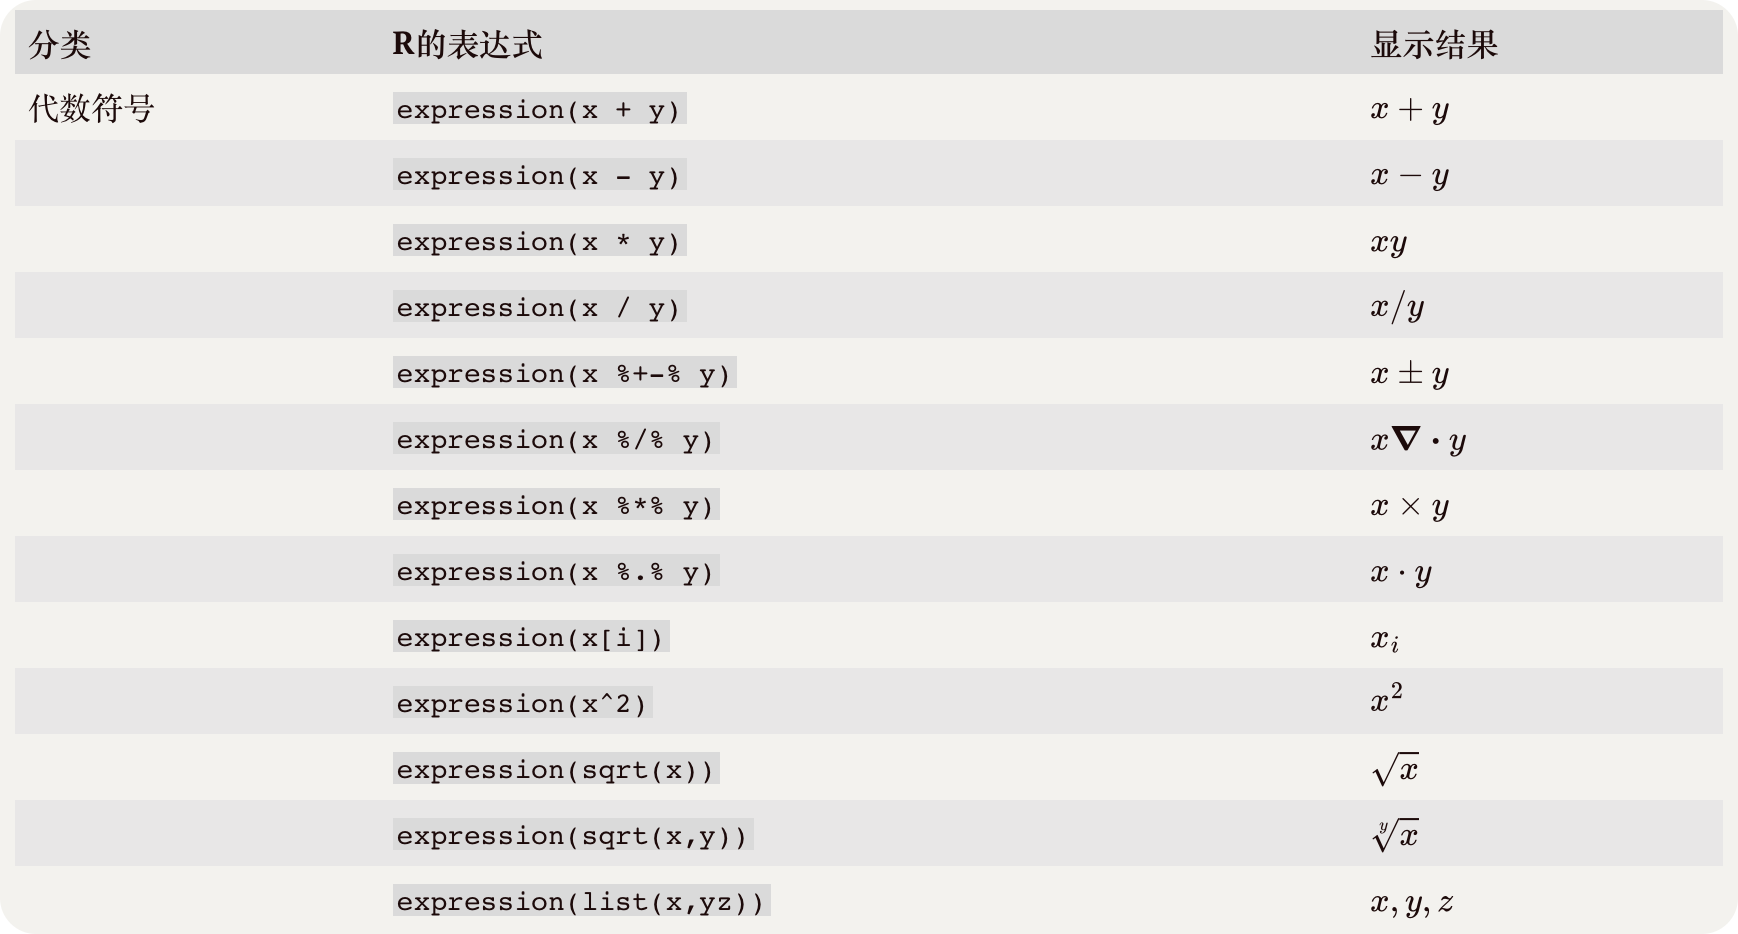
\includegraphics[width=0.8\textwidth]{/Users/lucas/Library/Mobile Documents/com~apple~CloudDocs/~~aa Study Materials/Grade 2 I/Learning/R for Data Science/Review of R/image/03_pic01.png}

\hypertarget{ux5e0cux814aux5b57ux7b26}{%
\subsubsection{希腊字符}\label{ux5e0cux814aux5b57ux7b26}}

\begin{Shaded}
\begin{Highlighting}[]
\FunctionTok{library}\NormalTok{(ggplot2);}
\NormalTok{greeks }\OtherTok{\textless{}{-}} \FunctionTok{c}\NormalTok{(}\StringTok{"Alpha"}\NormalTok{, }\StringTok{"Beta"}\NormalTok{, }\StringTok{"Gamma"}\NormalTok{, }\StringTok{"Delta"}\NormalTok{, }\StringTok{"Epsilon"}\NormalTok{, }\StringTok{"Zeta"}\NormalTok{,}
            \StringTok{"Eta"}\NormalTok{, }\StringTok{"Theta"}\NormalTok{, }\StringTok{"Iota"}\NormalTok{, }\StringTok{"Kappa"}\NormalTok{, }\StringTok{"Lambda"}\NormalTok{, }\StringTok{"Mu"}\NormalTok{,}
            \StringTok{"Nu"}\NormalTok{, }\StringTok{"Xi"}\NormalTok{, }\StringTok{"Omicron"}\NormalTok{, }\StringTok{"Pi"}\NormalTok{, }\StringTok{"Rho"}\NormalTok{, }\StringTok{"Sigma"}\NormalTok{,}
            \StringTok{"Tau"}\NormalTok{, }\StringTok{"Upsilon"}\NormalTok{, }\StringTok{"Phi"}\NormalTok{, }\StringTok{"Chi"}\NormalTok{, }\StringTok{"Psi"}\NormalTok{, }\StringTok{"Omega"}\NormalTok{);}

\NormalTok{dat }\OtherTok{\textless{}{-}} \FunctionTok{data.frame}\NormalTok{( }\AttributeTok{x =} \FunctionTok{rep}\NormalTok{( }\DecValTok{1}\SpecialCharTok{:}\DecValTok{6}\NormalTok{, }\DecValTok{4}\NormalTok{ ), }\AttributeTok{y =} \FunctionTok{rep}\NormalTok{( }\DecValTok{4}\SpecialCharTok{:}\DecValTok{1}\NormalTok{, }\AttributeTok{each =} \DecValTok{6}\NormalTok{), }\AttributeTok{greek =}\NormalTok{ greeks );}

\NormalTok{plot2 }\OtherTok{\textless{}{-}} 
  \FunctionTok{ggplot}\NormalTok{( dat, }\FunctionTok{aes}\NormalTok{(}\AttributeTok{x=}\NormalTok{x,}\AttributeTok{y=}\NormalTok{y) ) }\SpecialCharTok{+} \FunctionTok{geom\_point}\NormalTok{(}\AttributeTok{size =} \DecValTok{0}\NormalTok{) }\SpecialCharTok{+}
    \CommentTok{\# 画希腊字符,注意下面两行代码的区别}
    \FunctionTok{geom\_text}\NormalTok{( }\FunctionTok{aes}\NormalTok{( x, y }\SpecialCharTok{+} \FloatTok{0.1}\NormalTok{, }\AttributeTok{label =} \FunctionTok{tolower}\NormalTok{( greek ) ), }\AttributeTok{size =} \DecValTok{10}\NormalTok{, }\AttributeTok{parse =}\NormalTok{ T ) }\SpecialCharTok{+}
    \FunctionTok{geom\_text}\NormalTok{( }\FunctionTok{aes}\NormalTok{( x, y }\SpecialCharTok{{-}} \FloatTok{0.1}\NormalTok{, }\AttributeTok{label =} \FunctionTok{tolower}\NormalTok{( greek ) ), }\AttributeTok{size =} \DecValTok{5}\NormalTok{  );}
\end{Highlighting}
\end{Shaded}

\#\#

\begin{center}\rule{0.5\linewidth}{0.5pt}\end{center}

\newpage
\hypertarget{r-for-bioinformatics-data-summarisation-and-statistics}{%
\section{R for bioinformatics, data summarisation and
statistics}\label{r-for-bioinformatics-data-summarisation-and-statistics}}

\begin{quote}
Talk 10
\end{quote}

\hypertarget{toc-2}{%
\subsection{TOC}\label{toc-2}}

\begin{itemize}
\item
  Data summarisation functions (vector data)

  \begin{itemize}
  \item
    median, mean, sd, quantile, summary
  \end{itemize}
\item
  Graphical data summarisation (two-D data/ tibble/ table)

  \begin{itemize}
  \item
    dot plot
  \item
    smooth
  \item
    linear regression
  \item
    correlation \& variance explained
  \item
    groupping \& bar/ box/ plots
  \end{itemize}
\item
  statistics

  \begin{itemize}
  \item
    parametric tests

    \begin{itemize}
    \item
      t-test
    \item
      one way ANNOVA
    \item
      two way ANNOVA
    \item
      linear regression
    \item
      model / prediction / coefficients
    \end{itemize}
  \item
    non-parametric comparison
  \end{itemize}
\end{itemize}

\hypertarget{vector-summarization}{%
\subsection{Vector Summarization}\label{vector-summarization}}

\hypertarget{describe-normal-distribution}{%
\subsubsection{Describe Normal
Distribution}\label{describe-normal-distribution}}

You can use \texttt{mean} and \texttt{sd} to describe normal
distributions.

\begin{itemize}
\item
  是对称的。
\item
  均值和中位数是一样的。
\item
  最常见的值接近平均值;不太常见的价值观与之相去甚远。
\item
  标准差表示平均值到拐点的距离
\end{itemize}

\hypertarget{functions-to-generate-random-normal-distrubions}{%
\subsubsection{Functions to generate random normal
distrubions}\label{functions-to-generate-random-normal-distrubions}}

\begin{Shaded}
\begin{Highlighting}[]
\CommentTok{\# 生成 10000 个随机数字,使其 mean = 0, sd = 1,且为 normal distribution ...}
\NormalTok{x }\OtherTok{\textless{}{-}} \FunctionTok{rnorm}\NormalTok{(}\DecValTok{10000}\NormalTok{, }\AttributeTok{mean =} \DecValTok{0}\NormalTok{, }\AttributeTok{sd =} \DecValTok{1}\NormalTok{);}
\FunctionTok{ggplot}\NormalTok{( }\FunctionTok{data.frame}\NormalTok{( }\AttributeTok{data =}\NormalTok{ x ), }\FunctionTok{aes}\NormalTok{( data ) ) }\SpecialCharTok{+} \FunctionTok{geom\_density}\NormalTok{(  );}
\end{Highlighting}
\end{Shaded}

\hypertarget{other-regular-distributions}{%
\subsubsection{Other regular
distributions}\label{other-regular-distributions}}

\begin{enumerate}
\def\labelenumi{\arabic{enumi}.}
\item
  Uniform Distributions 均匀分布
\end{enumerate}

\begin{Shaded}
\begin{Highlighting}[]
\CommentTok{\# 为向量q中的值生成CDF概率 }
\FunctionTok{pnorm}\NormalTok{(q, }\AttributeTok{mean =} \DecValTok{0}\NormalTok{, }\AttributeTok{sd =} \DecValTok{1}\NormalTok{)    }

\CommentTok{\# 生成向量p中概率的分位数}
\FunctionTok{qnorm}\NormalTok{(p, }\AttributeTok{mean =} \DecValTok{0}\NormalTok{, }\AttributeTok{sd =} \DecValTok{1}\NormalTok{)    }

\CommentTok{\# 生成向量x中值的概率密度函数}
\FunctionTok{dnorm}\NormalTok{(x, }\AttributeTok{mean =} \DecValTok{0}\NormalTok{, }\AttributeTok{sd =} \DecValTok{1}\NormalTok{)}
\end{Highlighting}
\end{Shaded}

\begin{enumerate}
\def\labelenumi{\arabic{enumi}.}
\item
  Non-parametric Distributions 非参数分布

\begin{Shaded}
\begin{Highlighting}[]
\NormalTok{bi }\OtherTok{=}
	\FunctionTok{c}\NormalTok{(}\DecValTok{7}\NormalTok{, }\DecValTok{3}\NormalTok{, }\DecValTok{2}\NormalTok{, }\DecValTok{1}\NormalTok{, }\DecValTok{7}\NormalTok{, }
    \DecValTok{3}\NormalTok{, }\DecValTok{4}\NormalTok{, }\DecValTok{5}\NormalTok{, }\DecValTok{7}\NormalTok{, }\DecValTok{6}\NormalTok{,}
    \DecValTok{2}\NormalTok{, }\DecValTok{2}\NormalTok{, }\DecValTok{1}\NormalTok{, }\DecValTok{3}\NormalTok{, }\DecValTok{7}\NormalTok{, }
    \DecValTok{2}\NormalTok{, }\DecValTok{6}\NormalTok{, }\DecValTok{8}\NormalTok{, }\DecValTok{2}\NormalTok{, }\DecValTok{7}\NormalTok{,}
    \DecValTok{2}\NormalTok{, }\DecValTok{2}\NormalTok{, }\DecValTok{1}\NormalTok{, }\DecValTok{3}\NormalTok{, }\DecValTok{5}\NormalTok{, }
    \DecValTok{8}\NormalTok{, }\DecValTok{2}\NormalTok{, }\DecValTok{6}\NormalTok{, }\DecValTok{7}\NormalTok{, }\DecValTok{8}\NormalTok{, }
    \DecValTok{6}\NormalTok{, }\DecValTok{2}\NormalTok{, }\DecValTok{8}\NormalTok{, }\DecValTok{7}\NormalTok{, }\DecValTok{9}\NormalTok{, }
    \DecValTok{2}\NormalTok{, }\DecValTok{7}\NormalTok{, }\DecValTok{5}\NormalTok{, }\DecValTok{1}\NormalTok{, }\DecValTok{8}\NormalTok{, }
    \DecValTok{8}\NormalTok{, }\DecValTok{2}\NormalTok{, }\DecValTok{3}\NormalTok{, }\DecValTok{7}\NormalTok{, }\DecValTok{3}
\NormalTok{   )}
\FunctionTok{ggplot}\NormalTok{( }
  \FunctionTok{data.frame}\NormalTok{(}\AttributeTok{dat =}\NormalTok{ bi),}
  \FunctionTok{aes}\NormalTok{(dat)) }\SpecialCharTok{+} 
\FunctionTok{geom\_density}\NormalTok{()}
\end{Highlighting}
\end{Shaded}
\end{enumerate}

\hypertarget{uniform-distribution-ux7684ux5404ux79cdux51fdux6570}{%
\subsubsection{uniform distribution
的各种函数}\label{uniform-distribution-ux7684ux5404ux79cdux51fdux6570}}

注:以下函数中的 n 需要自行决定

\begin{Shaded}
\begin{Highlighting}[]
\CommentTok{\# generate n random numbers between 0 and 25}
\FunctionTok{runif}\NormalTok{(n, }\AttributeTok{min =} \DecValTok{0}\NormalTok{, }\AttributeTok{max =} \DecValTok{25}\NormalTok{)       }

\CommentTok{\# generate n random numbers between 0 and 25 (with replacement)}
\FunctionTok{sample}\NormalTok{(}\DecValTok{0}\SpecialCharTok{:}\DecValTok{25}\NormalTok{, n, }\AttributeTok{replace =} \ConstantTok{TRUE}\NormalTok{)   }

\CommentTok{\# generate n random numbers between 0 and 25 (without replacement)}
\FunctionTok{sample}\NormalTok{(}\DecValTok{0}\SpecialCharTok{:}\DecValTok{25}\NormalTok{, n, }\AttributeTok{replace =} \ConstantTok{FALSE}\NormalTok{)  }
\end{Highlighting}
\end{Shaded}

\hypertarget{other-distributions-cont}{%
\subsubsection{other distributions,
cont.}\label{other-distributions-cont}}

\begin{Shaded}
\begin{Highlighting}[]
\NormalTok{n }\OtherTok{\textless{}{-}} \DecValTok{10000}\NormalTok{;}
\NormalTok{uni }\OtherTok{\textless{}{-}} \FunctionTok{tibble}\NormalTok{( }\AttributeTok{dat =} \FunctionTok{runif}\NormalTok{(n), }\AttributeTok{type =} \StringTok{"uni"}\NormalTok{ );}
\NormalTok{norm }\OtherTok{\textless{}{-}} \FunctionTok{tibble}\NormalTok{( }\AttributeTok{dat =} \FunctionTok{rnorm}\NormalTok{(n), }\AttributeTok{type =} \StringTok{"norm"}\NormalTok{ );}
\NormalTok{binom }\OtherTok{\textless{}{-}} \FunctionTok{tibble}\NormalTok{( }\AttributeTok{dat =} \FunctionTok{rbinom}\NormalTok{(n, }\AttributeTok{size =} \DecValTok{100}\NormalTok{, }\AttributeTok{prob =} \FloatTok{0.5}\NormalTok{), }\AttributeTok{type =} \StringTok{"binom"}\NormalTok{ );}
\NormalTok{poisson }\OtherTok{\textless{}{-}} \FunctionTok{tibble}\NormalTok{( }\AttributeTok{dat =} \FunctionTok{rpois}\NormalTok{(n, }\AttributeTok{lambda =} \DecValTok{4}\NormalTok{), }\AttributeTok{type =} \StringTok{"poisson"}\NormalTok{ );}
\NormalTok{exp }\OtherTok{\textless{}{-}} \FunctionTok{tibble}\NormalTok{( }\AttributeTok{dat =} \FunctionTok{rexp}\NormalTok{(n, }\AttributeTok{rate =} \DecValTok{1}\NormalTok{) , }\AttributeTok{type =} \StringTok{"exp"}\NormalTok{);}
\NormalTok{gamma }\OtherTok{\textless{}{-}} \FunctionTok{tibble}\NormalTok{( }\AttributeTok{dat =} \FunctionTok{rgamma}\NormalTok{(n, }\AttributeTok{shape =} \DecValTok{1}\NormalTok{) , }\AttributeTok{type =} \StringTok{"gamma"}\NormalTok{);}
\end{Highlighting}
\end{Shaded}

\hypertarget{ux91cfux5316ux63cfux8ff0ux6570ux636e}{%
\subsubsection{量化描述数据}\label{ux91cfux5316ux63cfux8ff0ux6570ux636e}}

\begin{itemize}
\item
  \textbf{mean}: aka average, is the sum of all of the numbers in the
  data set divided by the size of the data set;
\item
  \textbf{median}: The median is the value that is in the middle when
  the numbers in a data set are sorted in increasing order;
\item
  \textbf{sd}: standard deviation;
\item
  \textbf{var}: measures how far a set of numbers are spread out;
\item
  \textbf{range}: range of values.
\end{itemize}

\hypertarget{ux91cfux5316ux63cfux8ff0ux51fdux6570}{%
\subsubsection{量化描述函数}\label{ux91cfux5316ux63cfux8ff0ux51fdux6570}}

\begin{Shaded}
\begin{Highlighting}[]
\FunctionTok{mean}\NormalTok{( norm}\SpecialCharTok{\$}\NormalTok{dat );}
\FunctionTok{median}\NormalTok{( norm}\SpecialCharTok{\$}\NormalTok{dat );}
  \FunctionTok{mode}\NormalTok{( norm}\SpecialCharTok{\$}\NormalTok{dat ); }\DocumentationTok{\#\# 确定给定对象的存储模式 "numeric", "character", "list" }

\FunctionTok{sd}\NormalTok{(norm}\SpecialCharTok{\$}\NormalTok{dat);}
\FunctionTok{var}\NormalTok{(norm}\SpecialCharTok{\$}\NormalTok{dat);}
\FunctionTok{range}\NormalTok{(norm}\SpecialCharTok{\$}\NormalTok{dat);}
\end{Highlighting}
\end{Shaded}

\hypertarget{quantile-and-summary}{%
\subsubsection{\texorpdfstring{\texttt{quantile} and
\texttt{summary}}{quantile and summary}}\label{quantile-and-summary}}

\begin{Shaded}
\begin{Highlighting}[]
\FunctionTok{quantile}\NormalTok{( norm}\SpecialCharTok{\$}\NormalTok{dat );}

\DocumentationTok{\#\# quantile 还接受其它参数 }
\FunctionTok{quantile}\NormalTok{( norm}\SpecialCharTok{\$}\NormalTok{dat, }\AttributeTok{probs =} \FunctionTok{seq}\NormalTok{(}\DecValTok{0}\NormalTok{, }\DecValTok{1}\NormalTok{, }\AttributeTok{length =} \DecValTok{11}\NormalTok{));}

\DocumentationTok{\#\# summary ... }
\FunctionTok{summary}\NormalTok{( norm}\SpecialCharTok{\$}\NormalTok{dat );}
\DocumentationTok{\#\# summary 也可应用于非数值}
\FunctionTok{summary}\NormalTok{( combined}\SpecialCharTok{\$}\NormalTok{type );}
\DocumentationTok{\#\# summary 可应用于整个表格; 相当于对每列进行 summary ... }
\FunctionTok{summary}\NormalTok{( combined );}
\end{Highlighting}
\end{Shaded}

\hypertarget{tableux51fdux6570}{%
\subsubsection{\texorpdfstring{\texttt{table}函数}{table函数}}\label{tableux51fdux6570}}

返回vector当中 unique 值和它们的出现次数

\hypertarget{count-in-dplyr}{%
\subsubsection{\texorpdfstring{\texttt{count} in \texttt{dplyr}
}{count in dplyr }}\label{count-in-dplyr}}

\hypertarget{ntile-ux51fdux6570ux7684ux53c2ux6570}{%
\subsubsection{\texorpdfstring{\texttt{ntile}
函数的参数}{ntile 函数的参数}}\label{ntile-ux51fdux6570ux7684ux53c2ux6570}}

... \texttt{*tile} 函数都是 equal size

\hypertarget{cut-ux51fdux6570}{%
\subsubsection{\texorpdfstring{\texttt{cut}
函数}{cut 函数}}\label{cut-ux51fdux6570}}

按指定的间隔 (breaks) 对数据进行分割。

不仅可用于 equal distance,还可以用于任意间距

\hypertarget{statistics}{%
\subsection{Statistics}\label{statistics}}

\hypertarget{parametric-tests}{%
\subsubsection{Parametric tests}\label{parametric-tests}}

parametric test 的要求

\begin{enumerate}
\def\labelenumi{\arabic{enumi}.}
\item
  随机取样
\item
  值或 residuals 为正态分布;residules 是指观察值与预测值(mean)之差
\item
  有相同的variance 方差
\end{enumerate}

\hypertarget{how-to-detect-outlier-}{%
\subsubsection{how to detect outlier ??}\label{how-to-detect-outlier-}}

一个很模糊的定义:Outliers are extreme values that fall a long way
outside of the other observations. For example, in a normal
distribution, outliers may be values on the tails of the distribution.

对于 normal distribution,通常 mean +- 2 or 3 * sd

IQR = s{[}"3rd Qu."{]}-s{[}"1st Qu."{]}

outlier: s{[}"1st Qu."{]} - 1.5 * IQR, s{[}"3rd Qu."{]} + 1.5 * IQR

\hypertarget{t-test}{%
\paragraph{\texorpdfstring{\texttt{t-test}}{t-test}}\label{t-test}}

检测分布是否与预期一致; e.g., whether the number of steps per day for
boys is significantly different from 10,000.

检验评估两个样本的均值是否有显著差异,假设样本服从正态分布,方差近似相等。

There are different types of t-tests in R, depending on the nature of
the comparison:

\begin{enumerate}
\def\labelenumi{\arabic{enumi}.}
\item
  \textbf{One-Sample t-test:}

  用于确定单个样本的均值与已知或假设的总体均值是否存在显著差异。

  Example:

\begin{Shaded}
\begin{Highlighting}[]
\NormalTok{RCopy code}
\NormalTok{\# One{-}sample t{-}test example}
\NormalTok{sample\_data = c(17, 21, 19, 23, 20, 18, 22)}
\NormalTok{t.test(sample\_data, mu = 20)}
\end{Highlighting}
\end{Shaded}

  This code performs a one-sample t-test on \texttt{sample\_data} to
  test if its mean differs significantly from 20.
\item
  \textbf{Independent Samples t-test (or Two-Sample t-test):}

  比较两个独立组的均值,以确定它们是否存在显著差异.

  Example:

\begin{Shaded}
\begin{Highlighting}[]
\NormalTok{RCopy code}
\NormalTok{\# Independent samples t{-}test example}
\NormalTok{group1 = c(23, 25, 28, 22, 20)}
\NormalTok{group2 = c(18, 21, 24, 19, 17)}
\NormalTok{t.test(group1, group2)}
\end{Highlighting}
\end{Shaded}

  This code performs an independent samples t-test on \texttt{group1}
  and \texttt{group2} to test if their means are significantly
  different.
\item
  \textbf{Paired t-test:}

  比较两个相关组的均值(例如,测量前和测量后),以确定它们是否有显著差异。

  Example:

\begin{Shaded}
\begin{Highlighting}[]
\NormalTok{RCopy code}
\NormalTok{\# Paired t{-}test example}
\NormalTok{before = c(32, 28, 30, 29, 31)}
\NormalTok{after = c(30, 25, 28, 27, 29)}
\NormalTok{t.test(before, after, paired = TRUE)}
\end{Highlighting}
\end{Shaded}

  This code performs a paired t-test on \texttt{before} and
  \texttt{after} to test if there\textquotesingle s a significant
  difference.
\end{enumerate}

The \texttt{t.test()} function in R is used to conduct these
t-tests.它返回检验统计量(t值)、自由度、p值和置信区间,从而深入了解观察到的差异是否具有统计显著性。

在R中执行t检验时,确保满足正态性和等方差的假设对于获得可靠的结果是很重要的。如果违反了这些假设,那么替代检验或数据转换可能更合适。

\hypertarget{one-way-annova}{%
\paragraph{One-way ANNOVA}\label{one-way-annova}}

In R, the one-way analysis of variance (ANOVA)
iS用于检验三个或三个以上独立(不相关)组的均数之间的显著差异。它评估这些群体的平均水平是否彼此显著不同。

The one-way ANOVA assumes that the data meet certain assumptions,
including:

\begin{itemize}
\item
  -正态性:每组应遵循正态分布。
\item
  -方差同质性:每组内的方差应大致相等。
\item
  -独立性:每组内的观测值应相互独立。
\end{itemize}

Here\textquotesingle s an example of performing a one-way ANOVA in R:

\begin{Shaded}
\begin{Highlighting}[]
\CommentTok{\# Example of one{-}way ANOVA}
\NormalTok{group1 }\OtherTok{=} \FunctionTok{c}\NormalTok{(}\DecValTok{15}\NormalTok{, }\DecValTok{20}\NormalTok{, }\DecValTok{25}\NormalTok{, }\DecValTok{30}\NormalTok{, }\DecValTok{35}\NormalTok{)}
\NormalTok{group2 }\OtherTok{=} \FunctionTok{c}\NormalTok{(}\DecValTok{10}\NormalTok{, }\DecValTok{18}\NormalTok{, }\DecValTok{25}\NormalTok{, }\DecValTok{32}\NormalTok{, }\DecValTok{40}\NormalTok{)}
\NormalTok{group3 }\OtherTok{=} \FunctionTok{c}\NormalTok{(}\DecValTok{12}\NormalTok{, }\DecValTok{22}\NormalTok{, }\DecValTok{28}\NormalTok{, }\DecValTok{32}\NormalTok{, }\DecValTok{38}\NormalTok{)}

\CommentTok{\# Combining data into a data frame}
\NormalTok{my\_data }\OtherTok{=} \FunctionTok{data.frame}\NormalTok{(}
  \AttributeTok{Values =} \FunctionTok{c}\NormalTok{(group1, group2, group3),}
  \AttributeTok{Group =} \FunctionTok{factor}\NormalTok{(}\FunctionTok{rep}\NormalTok{(}\DecValTok{1}\SpecialCharTok{:}\DecValTok{3}\NormalTok{, }\AttributeTok{each =} \DecValTok{5}\NormalTok{))  }\CommentTok{\# Creating a factor for groups}
\NormalTok{)}

\CommentTok{\# Performing one{-}way ANOVA}
\NormalTok{result\_anova }\OtherTok{=} \FunctionTok{aov}\NormalTok{(Values }\SpecialCharTok{\textasciitilde{}}\NormalTok{ Group, }\AttributeTok{data =}\NormalTok{ my\_data)}
\FunctionTok{summary}\NormalTok{(result\_anova)}
\end{Highlighting}
\end{Shaded}

Explanation of the code:

\begin{enumerate}
\def\labelenumi{\arabic{enumi}.}
\item
  The data for three groups (\texttt{group1}, \texttt{group2},
  \texttt{group3}) are created.
\item
  The data are combined into a data frame (\texttt{my\_data}) where the
  \texttt{Values} column contains the measurements and the
  \texttt{Group} column represents the group labels as a factor.
\item
  The \texttt{aov()} function is used to perform the one-way ANOVA,
  specifying the formula \texttt{Values\ \textasciitilde{}\ Group},
  indicating that \texttt{Values} is the dependent variable and
  \texttt{Group} is the independent variable.
\item
  \texttt{summary(result\_anova)} provides the ANOVA table with the
  F-statistic, degrees of freedom, p-value, and other relevant
  statistics.
\end{enumerate}

The output from \texttt{summary(result\_anova)} will
includeF-统计量、自由度、p-值和组内变异性,允许您确定组间均值是否有显著差异。

若p值小于选定的显著性水平(通常为0.05),则表明组均值之间存在显著差异。Additionally,
post-hoc tests like Tukey\textquotesingle s HSD test or pairwise t-tests
can be performed to identify which specific groups differ significantly
from each other after obtaining a significant result in the ANOVA.

\hypertarget{two-way-annova}{%
\paragraph{Two-way ANNOVA}\label{two-way-annova}}

A two-way analysis of variance (ANOVA) in R
用于检验两个分类自变量(因子)之间对连续因变量的交互作用效应。

Here\textquotesingle s an example:

\begin{Shaded}
\begin{Highlighting}[]
\CommentTok{\# Example of two{-}way ANOVA}
\CommentTok{\# Assume we have a dataset with \textquotesingle{}Treatment\textquotesingle{}, \textquotesingle{}Gender\textquotesingle{}, and \textquotesingle{}Response\textquotesingle{} variables}

\CommentTok{\# Creating sample data}
\FunctionTok{set.seed}\NormalTok{(}\DecValTok{123}\NormalTok{)}
\NormalTok{Treatment }\OtherTok{=} \FunctionTok{rep}\NormalTok{(}\FunctionTok{c}\NormalTok{(}\StringTok{"A"}\NormalTok{, }\StringTok{"B"}\NormalTok{, }\StringTok{"C"}\NormalTok{), }\AttributeTok{each =} \DecValTok{20}\NormalTok{)}
\NormalTok{Gender }\OtherTok{=} \FunctionTok{rep}\NormalTok{(}\FunctionTok{c}\NormalTok{(}\StringTok{"Male"}\NormalTok{, }\StringTok{"Female"}\NormalTok{), }\AttributeTok{times =} \DecValTok{30}\NormalTok{)}
\NormalTok{Response }\OtherTok{=} \FunctionTok{rnorm}\NormalTok{(}\DecValTok{60}\NormalTok{, }\AttributeTok{mean =} \FunctionTok{c}\NormalTok{(}\DecValTok{50}\NormalTok{, }\DecValTok{60}\NormalTok{, }\DecValTok{70}\NormalTok{), }\AttributeTok{sd =} \DecValTok{10}\NormalTok{)}

\CommentTok{\# Combining data into a data frame}
\NormalTok{my\_data }\OtherTok{=} \FunctionTok{data.frame}\NormalTok{(Treatment, Gender, Response)}

\CommentTok{\# Performing two{-}way ANOVA}
\NormalTok{result\_anova }\OtherTok{=} \FunctionTok{aov}\NormalTok{(Response }\SpecialCharTok{\textasciitilde{}}\NormalTok{ Treatment }\SpecialCharTok{+}\NormalTok{ Gender }\SpecialCharTok{+}\NormalTok{ Treatment}\SpecialCharTok{:}\NormalTok{Gender, }\AttributeTok{data =}\NormalTok{ my\_data)}
\FunctionTok{summary}\NormalTok{(result\_anova)}
\end{Highlighting}
\end{Shaded}

Explanation of the code:

\begin{enumerate}
\def\labelenumi{\arabic{enumi}.}
\item
  Sample data is created with three variables: \texttt{Treatment},
  \texttt{Gender}, and \texttt{Response}.
\item
  The data are combined into a data frame (\texttt{my\_data}), where
  \texttt{Treatment} and \texttt{Gender} are categorical factors, and
  \texttt{Response} is the continuous dependent variable.
\item
  The \texttt{aov()} function performs the two-way ANOVA. The formula
  \texttt{Response\ \textasciitilde{}\ Treatment\ +\ Gender\ +\ Treatment:Gender}
  specifies the main effects of \texttt{Treatment} and \texttt{Gender},
  as well as their interaction effect.
\item
  \texttt{summary(result\_anova)} provides the ANOVA table with
  F-statistics, degrees of freedom, p-values, and other statistics for
  each factor and their interaction.
\end{enumerate}

The output from \texttt{summary(result\_anova)} will
include治疗和性别的主要影响的信息,以及它们之间的交互作用效果。它支持您确定每个因子是否独立存在显著效应,以及它们的交互作用是否显著影响"响应"变量。

The interpretation of a two-way
ANOVA包括分析与每个因子及其交互作用相关联的p值。显著的p值表示相应的因子或交互作用对因变量有显著的影响。

Additionally, post-hoc tests or further analyses can be conducted to
explore specific comparisons between groups or factors after obtaining
significant results in the ANOVA.

\hypertarget{linear-regression}{%
\paragraph{Linear Regression}\label{linear-regression}}

线性回归是一种统计方法,通过对观测数据拟合线性方程来模拟因变量和一个或多个自变量之间的关系。

In R, linear regression can be performed using the \texttt{lm()}
function, which stands for "linear model."

Here\textquotesingle s an example:

\begin{Shaded}
\begin{Highlighting}[]
\CommentTok{\# Example of simple linear regression}
\CommentTok{\# Suppose we have a dataset with \textquotesingle{}x\textquotesingle{} as the independent variable and \textquotesingle{}y\textquotesingle{} as the dependent variable}

\CommentTok{\# Creating sample data}
\FunctionTok{set.seed}\NormalTok{(}\DecValTok{123}\NormalTok{)}
\NormalTok{x }\OtherTok{=} \DecValTok{1}\SpecialCharTok{:}\DecValTok{50}
\NormalTok{y }\OtherTok{=} \DecValTok{2} \SpecialCharTok{*}\NormalTok{ x }\SpecialCharTok{+} \FunctionTok{rnorm}\NormalTok{(}\DecValTok{50}\NormalTok{, }\AttributeTok{mean =} \DecValTok{0}\NormalTok{, }\AttributeTok{sd =} \DecValTok{5}\NormalTok{)  }\CommentTok{\# Generating \textquotesingle{}y\textquotesingle{} as a linear function of \textquotesingle{}x\textquotesingle{} with some noise}

\CommentTok{\# Creating a data frame}
\NormalTok{my\_data }\OtherTok{=} \FunctionTok{data.frame}\NormalTok{(x, y)}

\CommentTok{\# Performing linear regression}
\NormalTok{model }\OtherTok{=} \FunctionTok{lm}\NormalTok{(y }\SpecialCharTok{\textasciitilde{}}\NormalTok{ x, }\AttributeTok{data =}\NormalTok{ my\_data)}
\FunctionTok{summary}\NormalTok{(model)}
\end{Highlighting}
\end{Shaded}

Explanation of the code:

\begin{enumerate}
\def\labelenumi{\arabic{enumi}.}
\item
  Sample data is generated with an independent variable \texttt{x} and a
  dependent variable \texttt{y}. In this example, \texttt{y} is
  generated as a linear function of \texttt{x} with some added noise
  using \texttt{rnorm()} to simulate real-world variability.
\item
  The data are combined into a data frame \texttt{my\_data}.
\item
  The \texttt{lm()} function fits a linear regression model where
  \texttt{y} is the dependent variable and \texttt{x} is the independent
  variable (\texttt{y\ \textasciitilde{}\ x}). The argument
  \texttt{data\ =\ my\_data} specifies the data frame containing the
  variables.
\item
  \texttt{summary(model)} provides a summary of the linear regression
  model, including coefficients, standard errors, t-values, p-values,
  R-squared, and other statistics.
\end{enumerate}

Interpreting the output from \texttt{summary(model)}:

\begin{itemize}
\item
  The coefficients section shows the estimated coefficients for the
  intercept and the slope of the regression line (\texttt{Intercept} and
  \texttt{x}).
\item
  The p-values associated with the coefficients indicate the
  significance of each variable in predicting the dependent variable.
  Lower p-values suggest stronger evidence against the null hypothesis
  of no effect.
\item
  The R-squared value represents the proportion of variance in the
  dependent variable explained by the independent variable(s). Higher
  R-squared values indicate a better fit of the model to the data.
\end{itemize}

Linear regression in R can
also通过在模型中包含多个自变量,将其扩展到多元线性回归
(\texttt{y\ \textasciitilde{}\ x1\ +\ x2\ +\ ...}).

Additionally, diagnostic plots and further analyses can be performed to
assess model assumptions and goodness of fit.

\hypertarget{model--prediction--coefficients}{%
\paragraph{Model / Prediction /
Coefficients}\label{model--prediction--coefficients}}

In linear regression, the model equation is expressed as:

\begin{center}
	\([ y = \beta_0 + \beta_1 \cdot x_1 + \beta_2 \cdot x_2 + \ldots + \beta_n \cdot x_n + \epsilon ]\)
\end{center}


Where:

\begin{itemize}
\item
  ( \(y\) ) is the dependent variable.
\item
  (\( x_1, x_2, \ldots, x_n\) ) are the independent variables.
\item
  ( \( \beta_0\) ) is the intercept (constant term).
\item
  ( \( \beta_1, \beta_2, \ldots, \beta_n \) ) are the coefficients (slope
  parameters) that represent the change in ( \(  y  \) ) associated with a
  one-unit change in the corresponding ( \(  x  \) ) variable, assuming all
  other variables remain constant.
\item
  ( \(  \epsilon  \) ) represents the error term.
\end{itemize}

In R, after fitting a linear regression model using \texttt{lm()}:

\begin{Shaded}
\begin{Highlighting}[]
\CommentTok{\# Assuming \textquotesingle{}model\textquotesingle{} is the linear regression model obtained previously}
\FunctionTok{summary}\NormalTok{(model)}
\end{Highlighting}
\end{Shaded}

The output from \texttt{summary(model)} provides information including:

\begin{itemize}
\item
  \textbf{Coefficients:}
  本节显示每个自变量的估计系数("估计"),包括截距。这些系数代表因变量的估计变化,对应的自变量的一个单位的变化,保持其他变量不变。
\item
  \textbf{Residuals:}
  残差代表因变量的观测值和预测值之间的差异。这些用于评估模型的拟合优度。
\item
  \textbf{R-squared:}指示由自变量解释的因变量中的方差比例。较高的值指示模型对数据的拟合更好。
\end{itemize}

After obtaining the coefficients from the model, predictions can be made
using new or existing data:

\begin{Shaded}
\begin{Highlighting}[]
\CommentTok{\# Assuming \textquotesingle{}new\_data\textquotesingle{} contains the new data for prediction}
\NormalTok{predicted\_values }\OtherTok{=} \FunctionTok{predict}\NormalTok{(model, }\AttributeTok{newdata =}\NormalTok{ new\_data)}
\end{Highlighting}
\end{Shaded}

Replace \texttt{new\_data} with the data for which you want to make
predictions. The \texttt{predict()} function uses the coefficients from
the model to generate predicted values of the dependent variable based
on the independent variables in the new data.

The coefficients obtained from the linear regression model
(\texttt{model\$coefficients}) represent the slopes of the regression
line and the intercept, which are crucial for predicting new values and
understanding the relationships between variables in the model.

\hypertarget{non-parametric-comparison}{%
\subsubsection{Non-parametric
Comparison}\label{non-parametric-comparison}}

非参数方法是当参数方法所要求的正态性、方差齐性或线性假设被数据违反或不满足时所使用的统计技术。这些方法不依赖于特定的总体分布假设,对于分析可能不遵循正态分布的数据是有用的。

Here are some commonly used non-parametric methods for comparison in R:

\begin{enumerate}
\def\labelenumi{\arabic{enumi}.}
\item
  \textbf{Mann-Whitney U Test (Wilcoxon Rank-Sum Test):}

  用于在t检验的假设不满足时比较两个独立的组。

  Example:

\begin{Shaded}
\begin{Highlighting}[]
\CommentTok{\# Assuming \textquotesingle{}group1\textquotesingle{} and \textquotesingle{}group2\textquotesingle{} are vectors of numeric data}
\FunctionTok{wilcox.test}\NormalTok{(group1, group2)}
\end{Highlighting}
\end{Shaded}
\item
  \textbf{Kruskal-Wallis Test:}

  Mann-Whitney U检验的扩展,用于比较两个以上的独立组。

  Example:

\begin{Shaded}
\begin{Highlighting}[]
\CommentTok{\# Assuming \textquotesingle{}group1\textquotesingle{}, \textquotesingle{}group2\textquotesingle{}, \textquotesingle{}group3\textquotesingle{} are vectors of numeric data}
\FunctionTok{kruskal.test}\NormalTok{(}\FunctionTok{list}\NormalTok{(group1, group2, group3))}
\end{Highlighting}
\end{Shaded}
\item
  \textbf{Wilcoxon Signed-Rank Test:}

  用于比较配对样本或相关样本。

  Example:

\begin{Shaded}
\begin{Highlighting}[]
\CommentTok{\# Assuming \textquotesingle{}before\textquotesingle{} and \textquotesingle{}after\textquotesingle{} are vectors of paired numeric data}
\FunctionTok{wilcox.test}\NormalTok{(before, after, }\AttributeTok{paired =} \ConstantTok{TRUE}\NormalTok{)}
\end{Highlighting}
\end{Shaded}
\item
  \textbf{Mood\textquotesingle s Median Test:}

  测试两个或多个独立组中的中位数是否相等。

  Example:

\begin{Shaded}
\begin{Highlighting}[]
\CommentTok{\# Assuming \textquotesingle{}group1\textquotesingle{}, \textquotesingle{}group2\textquotesingle{}, \textquotesingle{}group3\textquotesingle{} are vectors of numeric data}
\NormalTok{median\_test }\OtherTok{=} \FunctionTok{mood.test}\NormalTok{(group1, group2, group3)}
\NormalTok{median\_test}
\end{Highlighting}
\end{Shaded}
\item
  \textbf{Friedman Test:}

  Wilcoxon Signed-Rank检验的扩展,用于比较两个以上配对或相关组。

  Example:

\begin{Shaded}
\begin{Highlighting}[]
\CommentTok{\# Assuming \textquotesingle{}group1\textquotesingle{}, \textquotesingle{}group2\textquotesingle{}, \textquotesingle{}group3\textquotesingle{} are matrices or data frames of paired numeric data}
\FunctionTok{friedman.test}\NormalTok{(group1, group2, group3)}
\end{Highlighting}
\end{Shaded}
\end{enumerate}

这些非参数检验提供了传统的参数检验的替代品,并对违反某些假设是强大的。它们在处理有序或倾斜数据或样本容量较小时特别有用,因为它们比参数检验依赖更少的分布假设。

\begin{center}\rule{0.5\linewidth}{0.5pt}\end{center}

\newpage
\hypertarget{linear-and-nonlinear-regression}{%
\section{Linear and nonlinear
regression}\label{linear-and-nonlinear-regression}}

\begin{quote}
Talk 11
\end{quote}

\textbf{This topic is particularly complex, so it is voluminous and
obscure.}

\hypertarget{toc-3}{%
\subsection{TOC}\label{toc-3}}

\begin{itemize}
\item
  linear regression
\item
  nonlinear regression
\item
  modeling and prediction
\item
  \textbf{K-fold} \& \textbf{X times} cross-validation
\item
  external validation
\end{itemize}

\hypertarget{linear-regression-2}{%
\subsection{Linear Regression}\label{linear-regression-2}}

\textbf{What is linear regression?}

线性回归是一种利用数理统计中的回归分析来确定两个或多个变量之间相互依赖的数量关系的统计分析方法。

\begin{itemize}
\item
  \texttt{Y} can be explained by a variable \texttt{X}: One-way Linear
  Regression
\item
  \texttt{Y} can be explained by multiple variables such as \texttt{X},
  \texttt{Z}: Multiple Linear Regression
\end{itemize}

Linear regression in R is typically performed using the \texttt{lm()}
function, which stands for "linear model." Here\textquotesingle s how to
fit a linear regression model in R and some useful functions related to
linear regression:

\hypertarget{fitting-a-linear-regression-model}{%
\subsubsection{Fitting a Linear Regression
Model:}\label{fitting-a-linear-regression-model}}

\begin{Shaded}
\begin{Highlighting}[]
\CommentTok{\# Example of fitting a linear regression model}
\CommentTok{\# Assuming \textquotesingle{}my\_data\textquotesingle{} is a data frame with \textquotesingle{}x\textquotesingle{} as the independent variable and \textquotesingle{}y\textquotesingle{} as the dependent variable}
\NormalTok{model }\OtherTok{=} \FunctionTok{lm}\NormalTok{(y }\SpecialCharTok{\textasciitilde{}}\NormalTok{ x, }\AttributeTok{data =}\NormalTok{ my\_data)}
\FunctionTok{summary}\NormalTok{(model)  }\CommentTok{\# Display summary statistics of the model}
\end{Highlighting}
\end{Shaded}

\begin{itemize}
\item
  \textbf{\texttt{lm()} Function:} Fits a linear regression model. The
  formula \texttt{y\ \textasciitilde{}\ x} specifies that \texttt{y} is
  the dependent variable and \texttt{x} is the independent variable.
  \texttt{data\ =\ my\_data} indicates the data frame containing the
  variables.
\item
  \textbf{\texttt{summary()} Function:} Displays a summary of the linear
  regression model, including coefficients, standard errors, t-values,
  p-values, R-squared, and other statistics.
\end{itemize}

\hypertarget{glm-vs-lm}{%
\subsubsection{\texorpdfstring{\texttt{glm} vs.
\texttt{lm}}{glm vs. lm}}\label{glm-vs-lm}}

\begin{Shaded}
\begin{Highlighting}[]
\NormalTok{lm(formula, data, …)}
\NormalTok{glm(formula, family=gaussian, data, …)}
\end{Highlighting}
\end{Shaded}

\textbf{glm}:

\begin{enumerate}
\def\labelenumi{\arabic{enumi}.}
\item
  当\texttt{family=gaussian}时,二者是一样的。
\end{enumerate}

\begin{Shaded}
\begin{Highlighting}[]
\FunctionTok{library}\NormalTok{(texreg);}
\NormalTok{m.lm }\OtherTok{\textless{}{-}} \FunctionTok{lm}\NormalTok{(am }\SpecialCharTok{\textasciitilde{}}\NormalTok{ disp }\SpecialCharTok{+}\NormalTok{ hp, }\AttributeTok{data=}\NormalTok{mtcars);}
\NormalTok{m.glm }\OtherTok{\textless{}{-}} \FunctionTok{glm}\NormalTok{(am }\SpecialCharTok{\textasciitilde{}}\NormalTok{ disp }\SpecialCharTok{+}\NormalTok{ hp, }\AttributeTok{data=}\NormalTok{mtcars);}
\FunctionTok{screenreg}\NormalTok{(}\AttributeTok{l =} \FunctionTok{list}\NormalTok{(m.lm, m.glm))}
\end{Highlighting}
\end{Shaded}

\hypertarget{glm-ux8fd8ux53efux7528ux4e8eux5176ux5b83ux7c7bux578bux6570ux636eux7684ux5206ux6790}{%
\subsubsection{\texorpdfstring{\texttt{glm}
还可用于其它类型数据的分析}{glm 还可用于其它类型数据的分析}}\label{glm-ux8fd8ux53efux7528ux4e8eux5176ux5b83ux7c7bux578bux6570ux636eux7684ux5206ux6790}}

\begin{enumerate}
\def\labelenumi{\arabic{enumi}.}
\item
  Logistic regression (family=binomial)
\end{enumerate}

预测的结果(Y)是binary的分类,比如\texttt{Yes},
\texttt{No},且只能有两个值;

\begin{Shaded}
\begin{Highlighting}[]
\NormalTok{dat }\OtherTok{\textless{}{-}}\NormalTok{ iris }\SpecialCharTok{\%\textgreater{}\%} \FunctionTok{filter}\NormalTok{( Species }\SpecialCharTok{\%in\%} \FunctionTok{c}\NormalTok{(}\StringTok{"setosa"}\NormalTok{, }\StringTok{"virginica"}\NormalTok{) );}
\NormalTok{bm }\OtherTok{\textless{}{-}} \FunctionTok{glm}\NormalTok{( Species }\SpecialCharTok{\textasciitilde{}}\NormalTok{ Sepal.Length }\SpecialCharTok{+}\NormalTok{ Sepal.Width }\SpecialCharTok{+}\NormalTok{ Petal.Length }\SpecialCharTok{+}\NormalTok{ Petal.Width, }
           \AttributeTok{data =}\NormalTok{ dat, }\AttributeTok{family =}\NormalTok{ binomial );}

\FunctionTok{data.frame}\NormalTok{( }\AttributeTok{predicted =}\NormalTok{ bm }\SpecialCharTok{\%\textgreater{}\%} \FunctionTok{predict}\NormalTok{( dat, }\AttributeTok{type =} \StringTok{"response"}\NormalTok{ ),}
            \AttributeTok{original =}\NormalTok{ dat}\SpecialCharTok{\$}\NormalTok{Species ) }\SpecialCharTok{\%\textgreater{}\%} \FunctionTok{sample\_n}\NormalTok{(}\DecValTok{6}\NormalTok{) }\SpecialCharTok{\%\textgreater{}\%} \FunctionTok{arrange}\NormalTok{( original );}
\end{Highlighting}
\end{Shaded}

\textbf{注意:}

\texttt{predict(.,\ type\ =\ "response")} 指示 \texttt{predict()}
函数返回模型的响应值。

对于逻辑回归模型,这意味着返回的是概率而不是对数几率。

\hypertarget{glmux7684poisson-regression-familypoisson}{%
\subsection{\texorpdfstring{\texttt{glm}的\texttt{Poisson\ regression\ (family=poisson)}}{glm的Poisson regression (family=poisson)}}\label{glmux7684poisson-regression-familypoisson}}

\textbf{泊松回归}是一种特殊类型的回归,其中响应变量由\textbf{计数数据组成}.

\textbf{Asumptions}:

\begin{enumerate}
\def\labelenumi{\arabic{enumi}.}
\item
  响应变量由计数数据组成。
\item
  观察是独立的。
\item
  模型的均值和方差相等。
\item
  计数的分布遵循泊松分布。
\end{enumerate}

\hypertarget{other-useful-functions-for-linear-regression-analysis}{%
\subsubsection{Other Useful Functions for Linear Regression
Analysis:}\label{other-useful-functions-for-linear-regression-analysis}}

\begin{enumerate}
\def\labelenumi{\arabic{enumi}.}
\item
  \textbf{\texttt{coefficients()} Function:}

  检索线性回归模型的系数。

  Example:

\begin{Shaded}
\begin{Highlighting}[]
\NormalTok{coef }\OtherTok{=} \FunctionTok{coefficients}\NormalTok{(model)}
\NormalTok{coef}
\end{Highlighting}
\end{Shaded}
\item
  \textbf{\texttt{predict()} Function:}

  使用拟合模型生成预测。

  Example:

\begin{Shaded}
\begin{Highlighting}[]
\NormalTok{new\_data }\OtherTok{=} \FunctionTok{data.frame}\NormalTok{(}\AttributeTok{x =} \FunctionTok{c}\NormalTok{(}\DecValTok{10}\NormalTok{, }\DecValTok{20}\NormalTok{, }\DecValTok{30}\NormalTok{))  }\CommentTok{\# New data for prediction}
\NormalTok{predicted\_values }\OtherTok{=} \FunctionTok{predict}\NormalTok{(model, }\AttributeTok{newdata =}\NormalTok{ new\_data)}
\NormalTok{predicted\_values}
\end{Highlighting}
\end{Shaded}
\item
  \textbf{\texttt{residuals()} Function:}

  检索残差(观测值和预测值之间的差异)。

  Example:

\begin{Shaded}
\begin{Highlighting}[]
\NormalTok{residuals }\OtherTok{=} \FunctionTok{residuals}\NormalTok{(model)}
\NormalTok{residuals}
\end{Highlighting}
\end{Shaded}
\item
  \textbf{\texttt{fitted()} Function:}

  检索拟合(预测)值。

  Example:

\begin{Shaded}
\begin{Highlighting}[]
\NormalTok{fitted\_values }\OtherTok{=} \FunctionTok{fitted}\NormalTok{(model)}
\NormalTok{fitted\_values}
\end{Highlighting}
\end{Shaded}
\item
  \textbf{\texttt{vcov()} Function:}

  计算系数的方差-协方差矩阵。

  Example:

\begin{Shaded}
\begin{Highlighting}[]
\NormalTok{var\_cov\_matrix }\OtherTok{=} \FunctionTok{vcov}\NormalTok{(model)}
\NormalTok{var\_cov\_matrix}
\end{Highlighting}
\end{Shaded}
\item
  \textbf{\texttt{anova()} Function:}

  对拟合模型执行方差分析(ANOVA)。

  Example:

\begin{Shaded}
\begin{Highlighting}[]
\NormalTok{anova\_table }\OtherTok{=} \FunctionTok{anova}\NormalTok{(model)}
\NormalTok{anova\_table}
\end{Highlighting}
\end{Shaded}
\item
  \textbf{\texttt{summary()} Function:}

  提供拟合模型的概述,包括参数估计值、标准误差、收敛信息和拟合优度统计量。

  Example:

\begin{Shaded}
\begin{Highlighting}[]
\FunctionTok{summary}\NormalTok{(model)}
\end{Highlighting}
\end{Shaded}
\item
  \textbf{\texttt{coef()} Function:}

  从拟合模型中提取估计系数。

  Example:

\begin{Shaded}
\begin{Highlighting}[]
\FunctionTok{coef}\NormalTok{(model)}
\end{Highlighting}
\end{Shaded}
\item
  \textbf{\texttt{confint()} Function (for prediction intervals):}

  计算拟合模型中预测值的预测区间。

  Example:

\begin{Shaded}
\begin{Highlighting}[]
\NormalTok{prediction\_intervals }\OtherTok{=} \FunctionTok{predict}\NormalTok{(model, }\AttributeTok{interval =} \StringTok{"prediction"}\NormalTok{)}
\NormalTok{prediction\_intervals}
\end{Highlighting}
\end{Shaded}
\item
  \textbf{\texttt{deviance()} Function:}

  计算拟合模型的偏差,这是缺乏拟合的度量。

  Example:

\begin{Shaded}
\begin{Highlighting}[]
\FunctionTok{deviance}\NormalTok{(model)}
\end{Highlighting}
\end{Shaded}
\item
  \textbf{\texttt{update()} Function:}

  允许使用不同的设置或数据更新或改装模型。

  Example:

\begin{Shaded}
\begin{Highlighting}[]
\NormalTok{updated\_model }\OtherTok{=} \FunctionTok{update}\NormalTok{(model, }\AttributeTok{start =} \FunctionTok{list}\NormalTok{(}\AttributeTok{a =} \DecValTok{2}\NormalTok{, }\AttributeTok{b =} \DecValTok{2}\NormalTok{, }\AttributeTok{c =} \DecValTok{2}\NormalTok{))}
\FunctionTok{summary}\NormalTok{(updated\_model)}
\end{Highlighting}
\end{Shaded}
\item
  \textbf{\texttt{AIC()} and \texttt{BIC()} Functions:}

  计算Akaike信息准则(阿灵顿资产投资)和贝叶斯信息准则(BIC)来评估模型质量和比较模型。

  Example:

\begin{Shaded}
\begin{Highlighting}[]
\FunctionTok{AIC}\NormalTok{(model)}
\FunctionTok{BIC}\NormalTok{(model)}
\end{Highlighting}
\end{Shaded}
\item
  \textbf{\texttt{plot()} Function (for diagnostic plots):}

  生成诊断图以评估模型的充分性(例如,残差与拟合值、Q-Q图)。

  Example:

\begin{Shaded}
\begin{Highlighting}[]
\FunctionTok{plot}\NormalTok{(model)}
\end{Highlighting}
\end{Shaded}
\end{enumerate}

These functions help in obtaining and analyzing various aspects of the
linear regression model, such as coefficients, predictions, residuals,
variance-covariance matrix, and ANOVA tables, aiding in model
interpretation, examining the fitted model\textquotesingle s statistics,
coefficients, goodness-of-fit measures, prediction intervals, model
comparisons, and diagnostics, allowing for a comprehensive analysis of
nonlinear regression models in R.

\hypertarget{nolinear-regression}{%
\subsection{Nolinear Regression}\label{nolinear-regression}}

当变量之间的关系不能用线性模型充分描述时,使用非线性回归。在R中,拟合非线性模型包括估计参数来描述变量之间的非线性关系。Here\textquotesingle s
an example using the \texttt{nls()} function, along with some relevant
functions for nonlinear regression analysis:

\hypertarget{fitting-a-nonlinear-regression-model}{%
\subsubsection{Fitting a Nonlinear Regression
Model:}\label{fitting-a-nonlinear-regression-model}}

\begin{enumerate}
\def\labelenumi{\arabic{enumi}.}
\item
  \texttt{nls(\ equation,\ data\ =\ data,\ start\ =\ ...\ )}
\item
  \texttt{y\textasciitilde{}a*x/(b+x)}
\end{enumerate}

\begin{Shaded}
\begin{Highlighting}[]
\CommentTok{\# Example of fitting a nonlinear regression model (assuming a quadratic function)}
\CommentTok{\# Assuming \textquotesingle{}my\_data\textquotesingle{} is a data frame with \textquotesingle{}x\textquotesingle{} as the independent variable and \textquotesingle{}y\textquotesingle{} as the dependent variable}

\CommentTok{\# Fitting a quadratic model: y = a * x\^{}2 + b * x + c}
\NormalTok{model }\OtherTok{=} \FunctionTok{nls}\NormalTok{(y }\SpecialCharTok{\textasciitilde{}}\NormalTok{ a }\SpecialCharTok{*} \FunctionTok{I}\NormalTok{(x}\SpecialCharTok{\^{}}\DecValTok{2}\NormalTok{) }\SpecialCharTok{+}\NormalTok{ b }\SpecialCharTok{*}\NormalTok{ x }\SpecialCharTok{+}\NormalTok{ c, }\AttributeTok{data =}\NormalTok{ my\_data, }\AttributeTok{start =} \FunctionTok{list}\NormalTok{(}\AttributeTok{a =} \DecValTok{1}\NormalTok{, }\AttributeTok{b =} \DecValTok{1}\NormalTok{, }\AttributeTok{c =} \DecValTok{1}\NormalTok{))}
\FunctionTok{summary}\NormalTok{(model)  }\CommentTok{\# Display summary statistics of the model}
\end{Highlighting}
\end{Shaded}

\begin{itemize}
\item
  \textbf{\texttt{nls()} Function:} Fits a nonlinear regression model.
  The formula
  \texttt{y\ \textasciitilde{}\ a\ *\ I(x\^{}2)\ +\ b\ *\ x\ +\ c}
  specifies a quadratic function. \texttt{data\ =\ my\_data} indicates
  the data frame containing the variables, and
  \texttt{start\ =\ list(a\ =\ 1,\ b\ =\ 1,\ c\ =\ 1)} provides initial
  parameter values.
\item
  \textbf{\texttt{summary()} Function:} Displays a summary of the
  nonlinear regression model, including parameter estimates, standard
  errors, t-values, convergence information, and other statistics.
\end{itemize}

\hypertarget{other-useful-functions-for-nonlinear-regression-analysis}{%
\subsubsection{Other Useful Functions for Nonlinear Regression
Analysis:}\label{other-useful-functions-for-nonlinear-regression-analysis}}

\begin{enumerate}
\def\labelenumi{\arabic{enumi}.}
\item
  \textbf{\texttt{predict()} Function:}

  Generates predictions using the fitted nonlinear model.

  Example:

\begin{Shaded}
\begin{Highlighting}[]
\NormalTok{new\_data }\OtherTok{=} \FunctionTok{data.frame}\NormalTok{(}\AttributeTok{x =} \FunctionTok{c}\NormalTok{(}\DecValTok{10}\NormalTok{, }\DecValTok{20}\NormalTok{, }\DecValTok{30}\NormalTok{))  }\CommentTok{\# New data for prediction}
\NormalTok{predicted\_values }\OtherTok{=} \FunctionTok{predict}\NormalTok{(model, }\AttributeTok{newdata =}\NormalTok{ new\_data)}
\NormalTok{predicted\_values}
\end{Highlighting}
\end{Shaded}
\item
  \textbf{\texttt{residuals()} Function:}

  Retrieves the residuals (differences between observed and predicted
  values).

  Example:

\begin{Shaded}
\begin{Highlighting}[]
\NormalTok{residuals }\OtherTok{=} \FunctionTok{residuals}\NormalTok{(model)}
\NormalTok{residuals}
\end{Highlighting}
\end{Shaded}
\item
  \textbf{\texttt{confint()} Function:}

  Computes confidence intervals for model parameters.

  Example:

\begin{Shaded}
\begin{Highlighting}[]
\NormalTok{conf\_intervals }\OtherTok{=} \FunctionTok{confint}\NormalTok{(model)}
\NormalTok{conf\_intervals}
\end{Highlighting}
\end{Shaded}
\item
  \textbf{\texttt{nls.control()} Function:}

  为\texttt{nls()}函数提供控制参数,允许对非线性拟合过程进行调整。

  Example:

\begin{Shaded}
\begin{Highlighting}[]
\NormalTok{control\_params }\OtherTok{=} \FunctionTok{nls.control}\NormalTok{(}\AttributeTok{maxiter =} \DecValTok{100}\NormalTok{, }\AttributeTok{tol =} \FloatTok{1e{-}6}\NormalTok{)}
\NormalTok{model }\OtherTok{=} \FunctionTok{nls}\NormalTok{(y }\SpecialCharTok{\textasciitilde{}}\NormalTok{ a }\SpecialCharTok{*} \FunctionTok{I}\NormalTok{(x}\SpecialCharTok{\^{}}\DecValTok{2}\NormalTok{) }\SpecialCharTok{+}\NormalTok{ b }\SpecialCharTok{*}\NormalTok{ x }\SpecialCharTok{+}\NormalTok{ c, }\AttributeTok{data =}\NormalTok{ my\_data, }\AttributeTok{start =} \FunctionTok{list}\NormalTok{(}\AttributeTok{a =} \DecValTok{1}\NormalTok{, }\AttributeTok{b =} \DecValTok{1}\NormalTok{, }\AttributeTok{c =} \DecValTok{1}\NormalTok{), }\AttributeTok{control =}\NormalTok{ control\_params)}
\end{Highlighting}
\end{Shaded}
\item
  \textbf{\texttt{anova()} Function:}

  Performs analysis of variance (ANOVA) for the fitted nonlinear model.

  Example:

\begin{Shaded}
\begin{Highlighting}[]
\NormalTok{anova\_table }\OtherTok{=} \FunctionTok{anova}\NormalTok{(model)}
\NormalTok{anova\_table}
\end{Highlighting}
\end{Shaded}
\item
  \textbf{\texttt{nlsLM()} Function (from the \texttt{minpack.lm}
  package):}

  \begin{itemize}
  \item
    An alternative to \texttt{nls()} that provides enhanced convergence
    properties and extended functionality for nonlinear least squares.
  \end{itemize}

  Example:

\begin{Shaded}
\begin{Highlighting}[]
\FunctionTok{library}\NormalTok{(minpack.lm)}
\NormalTok{model\_nlsLM }\OtherTok{=} \FunctionTok{nlsLM}\NormalTok{(y }\SpecialCharTok{\textasciitilde{}}\NormalTok{ a }\SpecialCharTok{*} \FunctionTok{I}\NormalTok{(x}\SpecialCharTok{\^{}}\DecValTok{2}\NormalTok{) }\SpecialCharTok{+}\NormalTok{ b }\SpecialCharTok{*}\NormalTok{ x }\SpecialCharTok{+}\NormalTok{ c, }\AttributeTok{data =}\NormalTok{ my\_data, }\AttributeTok{start =} \FunctionTok{list}\NormalTok{(}\AttributeTok{a =} \DecValTok{1}\NormalTok{, }\AttributeTok{b =} \DecValTok{1}\NormalTok{, }\AttributeTok{c =} \DecValTok{1}\NormalTok{))}
\FunctionTok{summary}\NormalTok{(model\_nlsLM)}
\end{Highlighting}
\end{Shaded}
\item
  \textbf{\texttt{augment()} Function (from the \texttt{broom}
  package):}

  \begin{itemize}
  \item
    使用其他列(如拟合/预测值、残差和其他模型信息)创建整洁的数据框架。
  \end{itemize}

  Example:

\begin{Shaded}
\begin{Highlighting}[]
\FunctionTok{library}\NormalTok{(broom)}
\NormalTok{augmented\_model }\OtherTok{=} \FunctionTok{augment}\NormalTok{(model)}
\FunctionTok{head}\NormalTok{(augmented\_model)}
\end{Highlighting}
\end{Shaded}
\item
  \textbf{\texttt{glance()} Function (from the \texttt{broom} package):}

  \begin{itemize}
  \item
    提取模型级统计信息,以简洁的格式提供模型的摘要。
  \end{itemize}

  Example:

\begin{Shaded}
\begin{Highlighting}[]
\NormalTok{glance\_summary }\OtherTok{=} \FunctionTok{glance}\NormalTok{(model)}
\NormalTok{glance\_summary}
\end{Highlighting}
\end{Shaded}
\item
  \textbf{\texttt{tidy()} Function (from the \texttt{broom} package):}

  \begin{itemize}
  \item
    将模型系数和相关统计数据提取到一个整洁的数据框架中。
  \end{itemize}

  Example:

\begin{Shaded}
\begin{Highlighting}[]
\NormalTok{tidy\_summary }\OtherTok{=} \FunctionTok{tidy}\NormalTok{(model)}
\NormalTok{tidy\_summary}
\end{Highlighting}
\end{Shaded}
\item
  \textbf{\texttt{nlstools::nlstools()} Function:}

  \begin{itemize}
  \item
    为非线性回归模型提供诊断工具和可视化,帮助模型评估。
  \end{itemize}

  Example:

\begin{Shaded}
\begin{Highlighting}[]
\FunctionTok{library}\NormalTok{(nlstools)}
\NormalTok{model\_tools }\OtherTok{=} \FunctionTok{nlstools}\NormalTok{(model)}
\FunctionTok{plot}\NormalTok{(model\_tools)}
\end{Highlighting}
\end{Shaded}
\item
  \textbf{\texttt{nls2()} Function:}

  \begin{itemize}
  \item
    提供具有多个起始值的\textquotesingle nls()\textquotesingle 的扩展版本,以改进收敛性。
  \end{itemize}

  Example:

\begin{Shaded}
\begin{Highlighting}[]
\NormalTok{model\_nls2 }\OtherTok{=} \FunctionTok{nls2}\NormalTok{(y }\SpecialCharTok{\textasciitilde{}}\NormalTok{ a }\SpecialCharTok{*} \FunctionTok{I}\NormalTok{(x}\SpecialCharTok{\^{}}\DecValTok{2}\NormalTok{) }\SpecialCharTok{+}\NormalTok{ b }\SpecialCharTok{*}\NormalTok{ x }\SpecialCharTok{+}\NormalTok{ c, }\AttributeTok{data =}\NormalTok{ my\_data, }\AttributeTok{start =} \FunctionTok{list}\NormalTok{(}\AttributeTok{a =} \DecValTok{1}\NormalTok{, }\AttributeTok{b =} \DecValTok{1}\NormalTok{, }\AttributeTok{c =} \DecValTok{1}\NormalTok{))}
\FunctionTok{summary}\NormalTok{(model\_nls2)}
\end{Highlighting}
\end{Shaded}
\end{enumerate}

These functions are commonly used for nonlinear regression analysis in
R, helping in prediction, residual analysis, confidence interval
computation, and controlling the fitting process.

\hypertarget{modeling-and-prediction}{%
\subsection{Modeling and Prediction}\label{modeling-and-prediction}}

When it comes to modeling and prediction using regression analysis,
especially nonlinear regression, understanding the model, making
predictions, and assessing the model\textquotesingle s performance are
crucial. Here\textquotesingle s a step-by-step guide on how to approach
modeling and prediction:

\hypertarget{modeling-and-prediction-steps}{%
\subsubsection{Modeling and Prediction
Steps:}\label{modeling-and-prediction-steps}}

\begin{enumerate}
\def\labelenumi{\arabic{enumi}.}
\item
  \textbf{Data Preparation:}
\end{enumerate}

Prepare your dataset with variables for the dependent (response) and
independent (predictor) variables.

\begin{enumerate}
\def\labelenumi{\arabic{enumi}.}
\item
  \textbf{Fitting the Nonlinear Model:}
\end{enumerate}

使用\texttt{nls()}或类似函数拟合非线性回归模型,指定适当的公式和初始参数值。

Example:

\begin{Shaded}
\begin{Highlighting}[]
\NormalTok{model }\OtherTok{=} 
\FunctionTok{nls}\NormalTok{(y }\SpecialCharTok{\textasciitilde{}}\NormalTok{ a }\SpecialCharTok{*} \FunctionTok{I}\NormalTok{(x}\SpecialCharTok{\^{}}\DecValTok{2}\NormalTok{) }\SpecialCharTok{+}\NormalTok{ b }\SpecialCharTok{*}\NormalTok{ x }\SpecialCharTok{+}\NormalTok{ c, }
    \AttributeTok{data =}\NormalTok{ my\_data,}
    \AttributeTok{start =} \FunctionTok{list}\NormalTok{(}\AttributeTok{a =} \DecValTok{1}\NormalTok{, }\AttributeTok{b =} \DecValTok{1}\NormalTok{, }\AttributeTok{c =} \DecValTok{1}\NormalTok{))}
\end{Highlighting}
\end{Shaded}

\begin{enumerate}
\def\labelenumi{\arabic{enumi}.}
\item
  \textbf{Model Summary and Assessment:}
\end{enumerate}

Use \texttt{summary()} and other functions (\texttt{glance()},
\texttt{tidy()}, etc.) 以获得模型的概述,包括系数、拟合优度度量和诊断。

Example:

\begin{Shaded}
\begin{Highlighting}[]
\FunctionTok{summary}\NormalTok{(model)}
\end{Highlighting}
\end{Shaded}

\begin{enumerate}
\def\labelenumi{\arabic{enumi}.}
\item
  \textbf{Prediction with the Fitted Model:}
\end{enumerate}

使用拟合模型为新数据或现有数据生成预测。

Example:

\begin{Shaded}
\begin{Highlighting}[]
\NormalTok{new\_data }\OtherTok{=} \FunctionTok{data.frame}\NormalTok{(}\AttributeTok{x =} \FunctionTok{c}\NormalTok{(}\DecValTok{10}\NormalTok{, }\DecValTok{20}\NormalTok{, }\DecValTok{30}\NormalTok{))  }\CommentTok{\# New data for prediction}
\NormalTok{predicted\_values }\OtherTok{=} \FunctionTok{predict}\NormalTok{(model, }\AttributeTok{newdata =}\NormalTok{ new\_data)}
\NormalTok{predicted\_values}
\end{Highlighting}
\end{Shaded}

\begin{enumerate}
\def\labelenumi{\arabic{enumi}.}
\item
  \textbf{Model Evaluation:}
\end{enumerate}

Evaluate the model\textquotesingle s performance using various metrics
(e.g., residuals, R-squared, RMSE) and diagnostic plots (e.g., residuals
vs. fitted values, Q-Q plots) to assess how well the model fits the
data.

\begin{enumerate}
\def\labelenumi{\arabic{enumi}.}
\item
  \textbf{Adjustment and Refinement:}
\end{enumerate}

Depending on the evaluation results, consider refining the model by
adjusting parameters, exploring different models, or including/excluding
variables to improve performance.

\begin{enumerate}
\def\labelenumi{\arabic{enumi}.}
\item
  \textbf{Prediction Intervals and Uncertainty:}
\end{enumerate}

Compute prediction intervals using \texttt{predict()} with
\texttt{interval\ =\ "prediction"} to quantify the uncertainty around
predictions.

\begin{enumerate}
\def\labelenumi{\arabic{enumi}.}
\item
  \textbf{Model Comparison (if applicable):}
\end{enumerate}

Compare multiple models using metrics like AIC, BIC, or likelihood ratio
tests to select the most appropriate model.

By following these steps, you\textquotesingle ll be able to build,
evaluate, and utilize nonlinear regression models for prediction in R
effectively. Remember, interpreting the model\textquotesingle s results,
assessing its assumptions, and validating predictions are crucial
aspects of regression analysis.

\hypertarget{k-fold--x-times-cross-validation}{%
\subsection{\texorpdfstring{\textbf{K-fold} \& \textbf{X times}
cross-validation}{K-fold \& X times cross-validation}}\label{k-fold--x-times-cross-validation}}

K-fold交叉验证和X次交叉验证都是用于评估机器学习模型(包括回归模型)的性能和泛化能力的技术,方法是将数据划分为子集进行训练和验证。

\hypertarget{k-fold-cross-validation}{%
\subsubsection{K-fold Cross-Validation:}\label{k-fold-cross-validation}}

k-fold交叉验证涉及将数据集拆分成K个大小相等的折叠。对模型进行K次训练,每次使用K-1折叠进行训练,其余折叠进行验证。这个过程确保每个数据点都用于训练和验证。

\hypertarget{steps-for-k-fold-cross-validation}{%
\paragraph{Steps for K-fold
Cross-Validation:}\label{steps-for-k-fold-cross-validation}}

\begin{enumerate}
\def\labelenumi{\arabic{enumi}.}
\item
  \textbf{Partition Data:} 将数据集分割成K个大小相等的折叠。
\item
  \textbf{Model Training:}
  对模型进行K次训练,每次使用K-1折叠作为训练数据。
\item
  \textbf{Validation:}验证模型在其余部分(训练中未使用)上的性能,并计算评估指标。.
\item
  \textbf{Average Metrics:}
  对K个迭代中的评估指标求平均值,以获得对模型性能的总体评估。
\end{enumerate}

\hypertarget{x-times-cross-validation}{%
\subsubsection{X times
Cross-Validation:}\label{x-times-cross-validation}}

X次交叉验证,也被称为重复的K-fold交叉验证,类似于K-fold的交叉验证,但这个过程是重复X次。它重复创建随机分区的数据到K折叠,训练模型,并评估其性能。该方法通过对多次试验的结果求平均值来提供更稳健的模型性能估计。

\hypertarget{steps-for-x-times-cross-validation}{%
\paragraph{Steps for X times
Cross-Validation:}\label{steps-for-x-times-cross-validation}}

\begin{enumerate}
\def\labelenumi{\arabic{enumi}.}
\item
  \textbf{Partition Data Repeatedly:} 将数据集随机分成K个折叠,X次。
\item
  \textbf{Model Training:} 为每个迭代训练模型,使用K-1折叠进行训练。
\item
  \textbf{Validation:} 验证模型在剩余折叠上的性能并计算评估指标。
\item
  \textbf{Average Metrics:}
  对X次迭代中的评估指标求平均值,以获得更稳定、更可靠的模型性能估计值。
\end{enumerate}

\hypertarget{implementation-in-r}{%
\subsubsection{Implementation in R:}\label{implementation-in-r}}

In R, you can perform K-fold and X times cross-validation using
functions from various packages like \texttt{caret}, \texttt{rsample},
or \texttt{crossval}. For example, using \texttt{caret}:

\hypertarget{k-fold-cross-validation-in-r-with-caret}{%
\paragraph{\texorpdfstring{K-fold Cross-Validation in R with
\texttt{caret}:}{K-fold Cross-Validation in R with caret:}}\label{k-fold-cross-validation-in-r-with-caret}}

\begin{Shaded}
\begin{Highlighting}[]
\FunctionTok{library}\NormalTok{(caret)}
\CommentTok{\# Define a train control using k{-}fold cross{-}validation}
\NormalTok{train\_control }\OtherTok{=}
	\FunctionTok{trainControl}\NormalTok{(}\AttributeTok{method =} \StringTok{"cv"}\NormalTok{, }\AttributeTok{number =}\NormalTok{ K)  }
\CommentTok{\# Specify K for the number of folds}

\CommentTok{\# Train the model using k{-}fold cross{-}validation}
\NormalTok{model }\OtherTok{=}
	\FunctionTok{train}\NormalTok{(}
\NormalTok{    formula, }
    \AttributeTok{data =}\NormalTok{ my\_data,}
    \AttributeTok{method =} \StringTok{"lm"}\NormalTok{,}
    \AttributeTok{trControl =}\NormalTok{ train\_control}
\NormalTok{  )}
\end{Highlighting}
\end{Shaded}

\hypertarget{x-times-cross-validation-in-r-with-caret}{%
\paragraph{\texorpdfstring{X times Cross-Validation in R with
\texttt{caret}:}{X times Cross-Validation in R with caret:}}\label{x-times-cross-validation-in-r-with-caret}}

\begin{Shaded}
\begin{Highlighting}[]
\FunctionTok{library}\NormalTok{(caret)}
\CommentTok{\# Define a train control using repeated k{-}fold cross{-}validation}
\NormalTok{train\_control }\OtherTok{=}
\FunctionTok{trainControl}\NormalTok{(}
  \AttributeTok{method =} \StringTok{"repeatedcv"}\NormalTok{,}
  \AttributeTok{number =}\NormalTok{ K, }\AttributeTok{repeats =}\NormalTok{ X) }
\CommentTok{\# Specify K for folds and X for repeats}

\CommentTok{\# Train the model using repeated k{-}fold cross{-}validation}
\NormalTok{model }\OtherTok{=}
	\FunctionTok{train}\NormalTok{(}
\NormalTok{    formula,}
    \AttributeTok{data =}\NormalTok{ my\_data,}
    \AttributeTok{method =} \StringTok{"lm"}\NormalTok{,}
    \AttributeTok{trControl =}\NormalTok{ train\_control}
\NormalTok{  )}
\end{Highlighting}
\end{Shaded}

Replace \texttt{formula} and \texttt{my\_data} with the appropriate
regression formula and your dataset. Adjust the parameters \texttt{K}
and \texttt{X} according to your preferences for the number of folds and
repetitions.

这些交叉验证技术有助于估计模型的性能,并帮助评估模型如何推广到看不见的数据,从而提供洞察其鲁棒性和可靠性。调整这些技术可以提高回归模型的准确性和稳定性的评价.

\hypertarget{external-validation}{%
\subsection{External Validation}\label{external-validation}}

外部验证是指使用在模型开发过程中未使用的独立数据集来评估预测模型的性能。它是评估一个模型如何从不同的来源或时间段推广到新的、看不见的数据的关键步骤,以验证它在实际应用中的可靠性和健壮性。

\hypertarget{steps-for-external-validation}{%
\subsubsection{Steps for External
Validation:}\label{steps-for-external-validation}}

\begin{enumerate}
\def\labelenumi{\arabic{enumi}.}
\item
  \textbf{Obtain an Independent Dataset:}
  获取与用于模型训练和验证的数据集不同的单独数据集。理想情况下,这个数据集应该代表相同的问题或领域,但来自不同的源、时间框架或人群。
\item
  \textbf{Preprocess Data:}
  对独立数据集进行类似于训练数据集的预处理(例如,处理缺失值、编码分类变量、缩放特征),以确保兼容性。
\item
  \textbf{Apply Trained Model:}
  使用在原始数据集上训练的模型对独立数据集进行预测。
\item
  \textbf{Evaluate Model Performance:}
  使用相关评估指标(例如准确度、RMSE、精度、召回率)评估模型在独立数据集上的性能,并将这些指标与在训练/验证数据集上实现的性能进行比较。
\item
  \textbf{Analyze Results:}
  分析从独立数据集获得的性能指标,以确定模型是否保持其预测能力和泛化能力。性能良好的独立数据集上的模型表明,良好的泛化能力和可靠性。
\end{enumerate}

\hypertarget{implementation-in-r-2}{%
\subsubsection{Implementation in R:}\label{implementation-in-r-2}}

In R, the process involves loading the trained model and applying it to
the independent dataset for prediction. Use appropriate evaluation
functions (\texttt{predict()}, evaluation metrics) to assess the
model\textquotesingle s performance on the external dataset.

\hypertarget{example-in-r}{%
\paragraph{Example in R:}\label{example-in-r}}

\begin{Shaded}
\begin{Highlighting}[]
\CommentTok{\# Load the trained model (replace \textquotesingle{}model\textquotesingle{} with your trained model)}
\FunctionTok{load}\NormalTok{(}\StringTok{"trained\_model.RData"}\NormalTok{)}

\CommentTok{\# Load and preprocess the independent dataset }
\CommentTok{\# (replace \textquotesingle{}independent\_data.csv\textquotesingle{} with your dataset)}
\NormalTok{independent\_data }\OtherTok{=} \FunctionTok{read.csv}\NormalTok{(}\StringTok{"independent\_data.csv"}\NormalTok{)}
\CommentTok{\# Perform similar preprocessing steps as used for the training data}

\CommentTok{\# Apply the trained model to the independent dataset for prediction}
\NormalTok{predicted\_values }\OtherTok{=} \FunctionTok{predict}\NormalTok{(model, }\AttributeTok{newdata =}\NormalTok{ independent\_data)}

\CommentTok{\# Evaluate model performance on the independent dataset}
\CommentTok{\# Use appropriate evaluation metrics }
\CommentTok{\# (e.g., RMSE, accuracy) }
\CommentTok{\# and compare with training/validation results}
\end{Highlighting}
\end{Shaded}

Replace the file paths, data loading, and evaluation steps with your
specific dataset and evaluation procedures. Ensure the compatibility of
the independent dataset with the preprocessing steps applied to the
original dataset for accurate evaluation.

\begin{center}\rule{0.5\linewidth}{0.5pt}\end{center}

\newpage
\hypertarget{machine-learning-basics}{%
\section{Machine learning basics}\label{machine-learning-basics}}

\begin{quote}
Talk 12
\end{quote}

\textbf{This topic is particularly complex, so it is voluminous and
obscure.}

\hypertarget{toc-4}{%
\subsection{TOC}\label{toc-4}}

\begin{itemize}
\item
  Machine Learning Algorithms Generalization
\item
  Random Forest
\item
  Feature Selection
\end{itemize}

\hypertarget{ux673aux5668ux5b66ux4e60ux53efux5206ux4e3aux4ee5ux4e0bux51e0ux7c7b}{%
\subsubsection{机器学习可分为以下几类}\label{ux673aux5668ux5b66ux4e60ux53efux5206ux4e3aux4ee5ux4e0bux51e0ux7c7b}}

\textbackslash FontSmall

1) \textbf{回归算法}

2) 基于实例的算法

3) \textbf{决策树学习}

4) 贝叶斯方法

5) 基于核的算法

6) \textbf{聚类算法}

7) \textbf{降低维度算法}

8) 关联规则学习

9) 集成算法

10) 人工神经网络

\hypertarget{1-ux56deux5f52ux7b97ux6cd5}{%
\subsubsection{1. 回归算法}\label{1-ux56deux5f52ux7b97ux6cd5}}

回归算法是试图采用对误差的衡量来探索变量之间的关系的一类算法。
常见的回归算法包括:

\begin{itemize}
\item
  最小二乘法(Ordinary Least Square),
\item
  逻辑回归(Logistic Regression) ,
\item
  逐步式回归(Stepwise Regression) ,
\item
  多元自适应回归样条(Multivariate Adaptive Regression Splines) 以及
\item
  本地散点平滑估计(Locally Estimated Scatterplot Smoothing)。
\end{itemize}

\hypertarget{2-ux57faux4e8eux5b9eux4f8bux7684ux7b97ux6cd5}{%
\subsubsection{2.
基于实例的算法}\label{2-ux57faux4e8eux5b9eux4f8bux7684ux7b97ux6cd5}}

基于实例的算法常常用来对决策问题建立模型,
这样的模型常常先选取一批样本数据,
然后根据某些近似性把新数据与样本数据进行比较。
通过这种方式来寻找最佳的匹配。

因此, 基于实例的算法常常也被称为``赢家通吃'' 学习或者``基于记忆的学习''
。 常见的算法包括:

\begin{itemize}
\item
  k-Nearest Neighbor(KNN),
\item
  学习矢量量化(Learning Vector Quantization, LVQ),以及
\item
  自组织映射算法(Self-Organizing Map, SOM) 。
\end{itemize}

深度学习的概念源于人工神经网络的研究。含多隐层的多层感知器就是一种深度学习结构。
深度学习通过组合低层特征形成更表示属性类别或特征,
以发现数据的分布式特征表示。

\hypertarget{3-ux51b3ux7b56ux6811ux5b66ux4e60}{%
\subsubsection{3. 决策树学习}\label{3-ux51b3ux7b56ux6811ux5b66ux4e60}}

决策树算法根据数据的属性采用树状结构建立决策模型,
决策树模型常常用来解决分类和回归问题。 常见的算法包括:

\begin{itemize}
\item
  分类及回归树(Classification And Regression Tree, CART) ,
\item
  ID3 (Iterative Dichotomiser 3),
\item
  C4.5, Chi-squared Automatic Interaction Detection(CHAID),
\item
  Decision Stump, 随机森林(Random Forest) ,
\item
  多元自适应回归样条(MARS)以及
\item
  梯度推进机(Gradient Boosting Machine, GBM) 。
\end{itemize}

\hypertarget{4-ux8d1dux53f6ux65afux65b9ux6cd5}{%
\subsubsection{4. 贝叶斯方法}\label{4-ux8d1dux53f6ux65afux65b9ux6cd5}}

贝叶斯方法算法是基于贝叶斯定理的一类算法, 主要用来解决分类和回归问题。
常见算法包括:

\begin{itemize}
\item
  朴素贝叶斯算法,
\item
  平均单依赖估计(Averaged One-Dependence Estimators,AODE) , 以及
\item
  Bayesian Belief Network(BBN) 。
\end{itemize}

\hypertarget{5-ux57faux4e8eux6838ux7684ux7b97ux6cd5}{%
\subsubsection{5.
基于核的算法}\label{5-ux57faux4e8eux6838ux7684ux7b97ux6cd5}}

基于核的算法中最著名的莫过于支持向量机(SVM) 了。
基于核的算法把输入数据映射到一个高阶的向量空间, 在这些高阶向量空间里,
有些分类或者回归问题能够更容易的解决。 常见的基于核的算法包括:

\begin{itemize}
\item
  支持向量机(Support Vector Machine, SVM) ,
\item
  径向基函数(Radial Basis Function, RBF), 以及
\item
  线性判别分析(Linear Discriminate Analysis,LDA)等。
\end{itemize}

\hypertarget{6-ux805aux7c7bux7b97ux6cd5}{%
\subsubsection{6. 聚类算法}\label{6-ux805aux7c7bux7b97ux6cd5}}

聚类, 就像回归一样, 有时候人们描述的是一类问题,
有时候描述的是一类算法。
聚类算法通常按照中心点或者分层的方式对输入数据进行归并。
所以的聚类算法都试图找到数据的内在结构,
以便按照最大的共同点将数据进行归类。 常见的聚类算法包括

\begin{itemize}
\item
  k-Means 算法以及
\item
  期望最大化算法(Expectation Maximization, EM) 。
\end{itemize}

\hypertarget{7-ux964dux4f4eux7ef4ux5ea6ux7b97ux6cd5}{%
\subsubsection{7.
降低维度算法}\label{7-ux964dux4f4eux7ef4ux5ea6ux7b97ux6cd5}}

像聚类算法一样, 降低维度算法试图分析数据的内在结构,
不过降低维度算法是以非监督学习的方式试图利用较少的信息来归纳或者解释数据。
这类算法可以用于高维数据的可视化或者用来简化数据以便监督式学习使用。
常见的算法包括:

\begin{itemize}
\item
  主成份分析(Principle Component Analysis, PCA) ,
\item
  偏最小二乘回归(Partial Least Square Regression, PLS) ,
\item
  Sammon 映射,
\item
  多维尺度(Multi-Dimensional Scaling, MDS) ,
\item
  投影追踪(Projection Pursuit)等。
\end{itemize}

\hypertarget{8-ux5173ux8054ux89c4ux5219ux5b66ux4e60}{%
\subsubsection{8.
关联规则学习}\label{8-ux5173ux8054ux89c4ux5219ux5b66ux4e60}}

关联规则学习通过寻找最能够解释数据变量之间关系的规则,
来找出大多元数据集中有用 联规则。 常见算法包括

\begin{itemize}
\item
  Apriori 算法和
\item
  Ec t 算法等。
\end{itemize}

\hypertarget{9-ux96c6ux6210ux7b97ux6cd5}{%
\subsubsection{9. 集成算法}\label{9-ux96c6ux6210ux7b97ux6cd5}}

集成算法用一些相对较弱的学习模型独立地就同样的样本进行训练,
然后把结果整合起来进行整体预测。
集成算法的主要难点在于究竟集成哪些独立的较弱的学习模型以及如何把学习结果整合起来。
这是一类非常强大的算法, 同时也非常流行。 常见的算法包括:

\begin{itemize}
\item
  Boosting,
\item
  Bootstrapped Aggregation(Bagging),
\item
  AdaBoost,
\item
  堆叠泛化(Stacked Generalization,Blending) ,
\item
  梯度推进机(Gradient Boosting Machine, GBM) ,
\item
  随机森林(Random Forest)
\end{itemize}

\hypertarget{10-ux4ebaux5de5ux795eux7ecfux7f51ux7edc}{%
\subsubsection{10.
人工神经网络}\label{10-ux4ebaux5de5ux795eux7ecfux7f51ux7edc}}

人工神经网络算法模拟生物神经网络, 是一类模式匹配算法。
通常用于解决分类和回归问题。 人工神经网络是机器学习的一个庞大的分支,
有几百种不同的算法。(其中\textbf{深度学习} 就是其中的一类算法) ,
重要的人工神经网络算法包括:

\begin{itemize}
\item
  感知器神经网络(Perceptron Neural Network) ,
\item
  反向传递(Back Propagation) ,
\item
  Hopfield 网络,
\item
  自组织映射(Self-Organizing Map, SOM) 。
\item
  学习矢量量化(Learning Vector Quantization, LVQ)。
\end{itemize}

\hypertarget{section-3-ux968fux673aux68eeux6797}{%
\subsubsection{section 3:
随机森林}\label{section-3-ux968fux673aux68eeux6797}}

\hypertarget{ux968fux673aux68eeux6797----random-forest}{%
\subsubsection{随机森林 -- Random
forest}\label{ux968fux673aux68eeux6797----random-forest}}

本文大部分内容取自``easyai.tech'' 网站的《随机森林 -- Random
forest》一文,有修改。

随机森林是一种由\textbf{决策树}构成的集成算法,适用于\textbf{小样本}数据,在很多情况下都能有不错的表现。

随机森林属于 \textbf{集成学习} 中的 Bagging(Bootstrap AGgregation
的简称) 方法。

\hypertarget{ux51b3ux7b56ux6811---decision-tree}{%
\subsection{决策树 - decision
tree}\label{ux51b3ux7b56ux6811---decision-tree}}

决策树是一种很简单的算法,他的解释性强,也符合人类的直观思维。这是一种基于if-then-else规则的有监督学习算法,

\hypertarget{steps-to-implement-random-forest-in-r}{%
\subsubsection{Steps to Implement Random Forest in
R:}\label{steps-to-implement-random-forest-in-r}}

\hypertarget{1-load-required-library}{%
\paragraph{\texorpdfstring{1. \textbf{Load Required
Library:}}{1. Load Required Library:}}\label{1-load-required-library}}

Start by loading the necessary library (\texttt{randomForest}) if not
already installed.

\begin{Shaded}
\begin{Highlighting}[]
\FunctionTok{install.packages}\NormalTok{(}\StringTok{"randomForest"}\NormalTok{)  }\CommentTok{\# Install package if not installed}
\FunctionTok{library}\NormalTok{(randomForest)}
\end{Highlighting}
\end{Shaded}

\hypertarget{2-prepare-data}{%
\paragraph{\texorpdfstring{2. \textbf{Prepare
Data:}}{2. Prepare Data:}}\label{2-prepare-data}}

将数据集加载到R中并执行必要的预处理步骤,如处理缺失值、对分类变量进行编码以及将数据拆分为训练集和测试集。

\begin{Shaded}
\begin{Highlighting}[]
\CommentTok{\# Example: Assuming \textquotesingle{}my\_data\textquotesingle{} is your dataset}
\CommentTok{\# Split data into features (X) and target variable (Y)}
\NormalTok{X }\OtherTok{=}\NormalTok{ my\_data[, }\SpecialCharTok{{-}}\NormalTok{target\_column\_index]  }\CommentTok{\# Features}
\NormalTok{Y }\OtherTok{=}\NormalTok{ my\_data[, target\_column\_index]   }\CommentTok{\# Target variable}
\end{Highlighting}
\end{Shaded}

\hypertarget{3-train-the-random-forest-model}{%
\paragraph{\texorpdfstring{3. \textbf{Train the Random Forest
Model:}}{3. Train the Random Forest Model:}}\label{3-train-the-random-forest-model}}

Use the \texttt{randomForest()} function to
通过指定公式和训练数据来训练模型。

\begin{Shaded}
\begin{Highlighting}[]
\CommentTok{\# Example: Training a Random Forest model for regression}
\NormalTok{model }\OtherTok{=} \FunctionTok{randomForest}\NormalTok{(Y }\SpecialCharTok{\textasciitilde{}}\NormalTok{ ., }\AttributeTok{data =}\NormalTok{ my\_data)}
\CommentTok{\# For classification: model = randomForest(factor(Y) \textasciitilde{} ., data = my\_data)}
\end{Highlighting}
\end{Shaded}

\hypertarget{4-model-tuning-optional}{%
\paragraph{\texorpdfstring{4. \textbf{Model Tuning
(Optional):}}{4. Model Tuning (Optional):}}\label{4-model-tuning-optional}}

Adjust hyperparameters such as the number of trees (\texttt{ntree}),
maximum depth (\texttt{max\_depth}), and others to optimize model
performance.

\begin{Shaded}
\begin{Highlighting}[]
\CommentTok{\# Example: Setting number of trees and maximum depth}
\NormalTok{model }\OtherTok{=} \FunctionTok{randomForest}\NormalTok{(Y }\SpecialCharTok{\textasciitilde{}}\NormalTok{ ., }\AttributeTok{data =}\NormalTok{ my\_data, }\AttributeTok{ntree =} \DecValTok{100}\NormalTok{, }\AttributeTok{max\_depth =} \DecValTok{10}\NormalTok{)}
\end{Highlighting}
\end{Shaded}

\hypertarget{5-make-predictions}{%
\paragraph{\texorpdfstring{5. \textbf{Make
Predictions:}}{5. Make Predictions:}}\label{5-make-predictions}}

Use the trained model to make predictions on new or test data.

\begin{Shaded}
\begin{Highlighting}[]
\CommentTok{\# Example: Making predictions on test data}
\NormalTok{predicted\_values }\OtherTok{=} \FunctionTok{predict}\NormalTok{(model, }\AttributeTok{newdata =}\NormalTok{ test\_data)}
\end{Highlighting}
\end{Shaded}

\hypertarget{6-model-evaluation}{%
\paragraph{\texorpdfstring{6. \textbf{Model
Evaluation:}}{6. Model Evaluation:}}\label{6-model-evaluation}}

Evaluate the model\textquotesingle s performance using appropriate
metrics (e.g., RMSE for regression, accuracy, confusion matrix for
classification) on test/validation data.

\begin{Shaded}
\begin{Highlighting}[]
\CommentTok{\# Example: Evaluate model performance (for regression)}
\NormalTok{error }\OtherTok{=} \FunctionTok{sqrt}\NormalTok{(}\FunctionTok{mean}\NormalTok{((predicted\_values }\SpecialCharTok{{-}}\NormalTok{ true\_values)}\SpecialCharTok{\^{}}\DecValTok{2}\NormalTok{))  }\CommentTok{\# Calculate RMSE}
\end{Highlighting}
\end{Shaded}

\hypertarget{example---random-forest-for-regression}{%
\subsubsection{Example - Random Forest for
Regression:}\label{example---random-forest-for-regression}}

Here\textquotesingle s an example using a built-in dataset
(\texttt{mtcars}) in R for regression:

\begin{Shaded}
\begin{Highlighting}[]
\FunctionTok{library}\NormalTok{(randomForest)}

\CommentTok{\# Load dataset}
\FunctionTok{data}\NormalTok{(mtcars)}

\CommentTok{\# Split data into features and target variable}
\NormalTok{X }\OtherTok{=}\NormalTok{ mtcars[, }\SpecialCharTok{{-}}\DecValTok{1}\NormalTok{]  }\CommentTok{\# Exclude the first column (target variable)}
\NormalTok{Y }\OtherTok{=}\NormalTok{ mtcars[, }\DecValTok{1}\NormalTok{]   }\CommentTok{\# First column (target variable)}

\CommentTok{\# Train the Random Forest model}
\NormalTok{model }\OtherTok{=} \FunctionTok{randomForest}\NormalTok{(Y }\SpecialCharTok{\textasciitilde{}}\NormalTok{ ., }\AttributeTok{data =}\NormalTok{ mtcars)}

\CommentTok{\# Make predictions on the same dataset (for demonstration)}
\NormalTok{predicted\_values }\OtherTok{=} \FunctionTok{predict}\NormalTok{(model, }\AttributeTok{newdata =}\NormalTok{ mtcars)}

\CommentTok{\# Evaluate model performance (RMSE)}
\NormalTok{error }\OtherTok{=} \FunctionTok{sqrt}\NormalTok{(}\FunctionTok{mean}\NormalTok{((predicted\_values }\SpecialCharTok{{-}}\NormalTok{ mtcars}\SpecialCharTok{\$}\NormalTok{mpg)}\SpecialCharTok{\^{}}\DecValTok{2}\NormalTok{))}
\end{Highlighting}
\end{Shaded}

Replace \texttt{my\_data}, \texttt{test\_data}, and the respective
column names with your specific dataset and target variable. Adjust
hyperparameters based on your problem and dataset characteristics for
better model performance. Additionally, use appropriate evaluation
metrics for assessing model accuracy and performance.

\hypertarget{feature-selection}{%
\subsection{Feature Selection}\label{feature-selection}}

特征选择是机器学习中的一个关键步骤,旨在选择最相关、最具信息量的特征,以提高模型性能、降低计算复杂度并减轻过拟合。在R中,各种方法可以帮助识别重要的特征。

\hypertarget{feature-selection-techniques-in-r}{%
\subsubsection{Feature Selection Techniques in
R:}\label{feature-selection-techniques-in-r}}

\hypertarget{1-correlation-analysis}{%
\paragraph{\texorpdfstring{1. \textbf{Correlation
Analysis:}}{1. Correlation Analysis:}}\label{1-correlation-analysis}}

计算特征与目标变量之间或特征本身之间的相关系数,以识别高度相关的特征。删除冗余或高度相关的功能。

\begin{Shaded}
\begin{Highlighting}[]
\CommentTok{\# Example: Using cor() for correlation analysis}
\NormalTok{correlation\_matrix }\OtherTok{=} \FunctionTok{cor}\NormalTok{(my\_data)}
\end{Highlighting}
\end{Shaded}

\hypertarget{2-filter-methods}{%
\paragraph{\texorpdfstring{2. \textbf{Filter
Methods:}}{2. Filter Methods:}}\label{2-filter-methods}}

使用统计方法(例如,卡方检验,互信息),以排名和选择的基础上,他们的个人相关的目标变量的功能。

\begin{Shaded}
\begin{Highlighting}[]
\CommentTok{\# Example: Using chi{-}squared test for feature selection}
\FunctionTok{library}\NormalTok{(caret)}
\NormalTok{feature\_selection }\OtherTok{=} \FunctionTok{nearZeroVar}\NormalTok{(my\_data)}
\end{Highlighting}
\end{Shaded}

\hypertarget{3-wrapper-methods}{%
\paragraph{\texorpdfstring{3. \textbf{Wrapper
Methods:}}{3. Wrapper Methods:}}\label{3-wrapper-methods}}

通过迭代训练模型并选择可实现最佳模型性能的子集来评估特征子集。

\begin{Shaded}
\begin{Highlighting}[]
\CommentTok{\# Example: Using recursive feature elimination (RFE)}
\FunctionTok{library}\NormalTok{(caret)}
\NormalTok{control }\OtherTok{=} \FunctionTok{rfeControl}\NormalTok{(}\AttributeTok{functions =}\NormalTok{ rfFuncs, }\AttributeTok{method =} \StringTok{"cv"}\NormalTok{, }\AttributeTok{number =} \DecValTok{10}\NormalTok{)}
\NormalTok{feature\_selection }\OtherTok{=} \FunctionTok{rfe}\NormalTok{(X, Y, }\AttributeTok{sizes =} \FunctionTok{c}\NormalTok{(}\DecValTok{1}\SpecialCharTok{:}\DecValTok{10}\NormalTok{), }\AttributeTok{rfeControl =}\NormalTok{ control)}
\end{Highlighting}
\end{Shaded}

\hypertarget{4-embedded-methods}{%
\paragraph{\texorpdfstring{4. \textbf{Embedded
Methods:}}{4. Embedded Methods:}}\label{4-embedded-methods}}

模型训练期间的特征选择,其中算法本身执行特征选择(例如,LASSO、随机森林、梯度提升)。

\begin{Shaded}
\begin{Highlighting}[]
\CommentTok{\# Example: Using Random Forest for feature selection}
\FunctionTok{library}\NormalTok{(randomForest)}
\NormalTok{model }\OtherTok{=} \FunctionTok{randomForest}\NormalTok{(Y }\SpecialCharTok{\textasciitilde{}}\NormalTok{ ., }\AttributeTok{data =}\NormalTok{ my\_data)}
\NormalTok{importance }\OtherTok{=} \FunctionTok{importance}\NormalTok{(model)}
\end{Highlighting}
\end{Shaded}

\hypertarget{5-dimensionality-reduction-techniques}{%
\paragraph{\texorpdfstring{5. \textbf{Dimensionality Reduction
Techniques:}}{5. Dimensionality Reduction Techniques:}}\label{5-dimensionality-reduction-techniques}}

主成分分析(PCA)或t-Distributed随机近邻嵌入(t-SNE)等技术通过创建捕获大部分原始信息的新变量来缩小特征空间。

\begin{Shaded}
\begin{Highlighting}[]
\CommentTok{\# Example: PCA for feature reduction}
\NormalTok{pca\_result }\OtherTok{=} \FunctionTok{prcomp}\NormalTok{(my\_data, }\AttributeTok{scale. =} \ConstantTok{TRUE}\NormalTok{)}
\end{Highlighting}
\end{Shaded}

根据数据集的特征、问题复杂性和计算资源选择特征选择方法。多种技术的组合通常会产生最好的结果,因为不同的方法可以捕获特征重要性的不同方面。进行试验和迭代,为您的机器学习模型找到最适合的功能。

\begin{center}\rule{0.5\linewidth}{0.5pt}\end{center}

\textbf{This is the end of the article. Take a rest\textasciitilde{}}

\end{document}
